\chapter{Prototype Construction and Testing}
\label{chap:ProtoTypeBuildTest}
%This chapter will detail the process of integrating the three parts of the WHIPPED system together to make an end-to-end application. I will first discuss integrating the smartphone and sensor suite to gather physiometric data. Then discuss the integration of the smartphone and BKE, separate from the sensors, to communicate psychosocial information. Finally, I will discuss the BKE‘s integration of all knowledge from both the sensors, via the smartphone, and the psychosocial data to calculate wellness and provide interventions.

%i apologize for the 62 times i use the word module.

This chapter covers the Hardware design and unit testing of the Wireless Health indicator patch (WHIP) and its initial construction. The different modules of the final prototype are outlined and their overall integration discussed, Procedures for testing the functionality of the design in a laboratory environment are discussed. Next, the physical design of the sensor apparatus is covered.

\section{Electronic design}


The core of the dissertation is the Wireless Health Indicator Patch (WHIP). This device, if properly connected to a patient, records all the needed data to derive the metrics described in \nameref{chap:SensorConcepts} and stores this data to a Secure Digital (SD) card for later retrieval. Additional functionality is offered via a Bluetooth (BT) connection. The final device used for the trial is the fifth revision of designs dating back to 2011. Details on previous versions can be found in \nameref{sec:ResearchDoneToDate}. The remainder of this section focuses on the final prototype.

The WHIP device consists of several modules, interacting across a standard communication buses. Each device is discussed including the power-module, the Memory-module, the ECG-module, the \spo2-module, the Communication-module, and finally the control-module. Once each module is fully defined the methods for integration are covered. Many of the modules have evolved from the first prototype, starting as simple fixed modules and becoming more configurable at the expense of an increased component count and complexity. The final prototype consists of many modules with only a singe chip or device handling all the details of the module internally, as in the case of the ECG, \spo2, SD card, and Bluetooth modules. The important part of defining each module is to specify the inputs and outputs of each module as well as any protocols used to communicate with the device.

\subsection {The Schematic Capture}
The following sections discuss different modules that were synthesized for the Whip sensor. These schematics were created in Cadsoft eagleCAD (Eagle)\cite{Eagle2017} a schematic capture and layout program. Eagle was used to both layout the schematic and PCB. The full schematic is included in \cref{chap:PCB_Schematics}, however, figures for each module are included below.

\subsubsection {The Power Module}
\begin{figure}
	\begin{center}
		\label{fig:Rev5_power}
		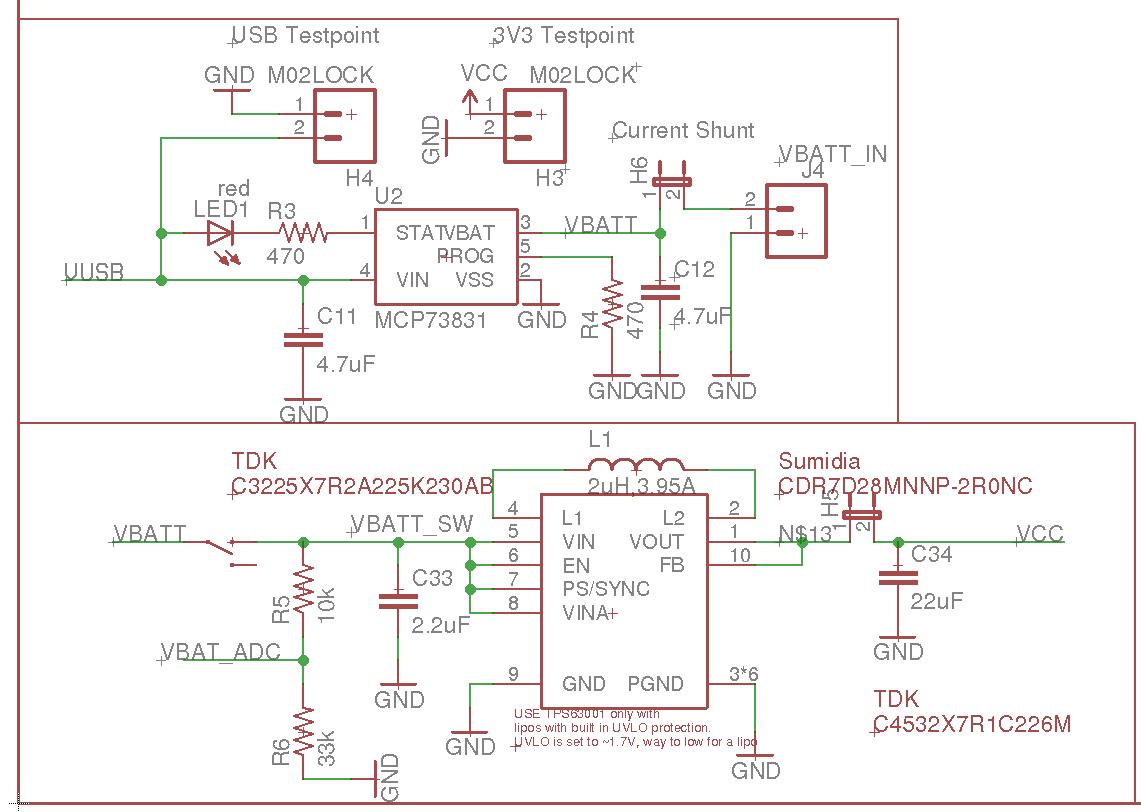
\includegraphics[scale=1,width=0.9\textwidth]{Images/Rev5_PowerSch.png} 
		\caption{Power supply and charging circuit for Whip Sensor}
	\end{center}
\end{figure}

\Cref{fig:Rev5_power} shows the schematic for the power module, responsible for providing power to all other modules. All modules are configured to operate at 3.3 Volts to simplify design. The other requirement for the power module is the ability to operate from, and charge, a single cell lithium polymer (LiPo) battery. Ultimately a design based on an existing open source power module was constructed \cite{Sparkfun2012}. Modifications to the Open Source HardWare(OSHW) design increased the current carrying capacity, and inflated the charging rate.

The power and charging design was featured on every WHIP prototype starting with version 1. The regulator circuit is based around the TPS61200 family of Buck/Boost regulators\cite{TPS610X}, this IC will provide a regulated 3.3V output over the entire range of a LiPo's voltage range, roughly 4.2 to 2.9 volts. Battery charging is handled by the MCP73831, a monolithic charge handler\cite{MCP73831}. The MCP73831 converts USB power, when available, to an appropriate charge voltage. The module uses a two pin keyed JST connector for connection to the battery and mini USB is used to provide power to charge the battery. Mini-USB was chosen over Micro-USB with the assumption that it would be easier for sight impaired users to correctly plug the device in. the power module also provides informational signals to the control module about battery health and charge status.

%JST doesnt stand for anything its the name of the company... %

\subsubsection {The Memory Module}
\begin{figure}
	\begin{center}
		\label{fig:Rev5_SDCARD}
		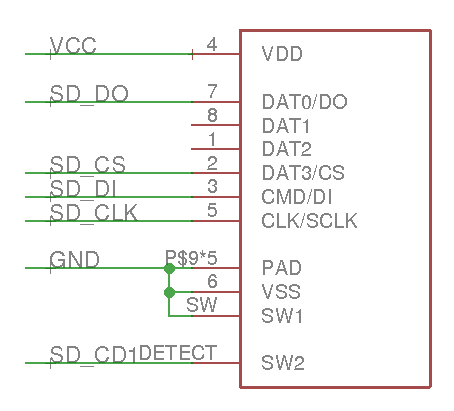
\includegraphics[scale=1,width=0.5\textwidth]{Images/Rev5_SDCARD.png} 
		\caption{Memory Circuit connections for Whip Sensor}
	\end{center}
\end{figure}
The Memory module is responsible for saving all patient biometric data. The device chosen was a micro SD card. The first revision of the WHIP board included a full sized SD card was as a trial of the technology. A micro SD card was used in the final prototype to reduce device size. The interface, shown in \cref{fig:Rev5_SDCARD}, remains the same regardless of card configuration. SD cards can communicate using the Serial Peripheral interface (SPI). SPI is a de facto standard, no standards body maintains the specification of SPI. SPI uses 4 wires to provide a full duplex synchronous communication channel. The memory module for the WHIP is actually the SD card, the only other part of the module is the card socket. All read and write logic is handled by the circuitry on the card. Offloading the flash algorithms to an sd card greatly simplifies the board design. However, SD cards are not 5 Volt tolerant this was part of the reason the power module provides 3.3V. The SPI bus for the memory module allows the control module to use a full FAT32 file system on the SD card using only the SPI interface.

In the Eagle the SD card device was created as a custom component and footprint. Then, to simplify the schematic diagrams off-page connectors were used to create a logical connection to the processor unit without cluttering the system diagram with excessive net wires.

\subsubsection{The ECG Module}
\begin{figure}
	\begin{center}
		\label{fig:Rev5_ECG}
		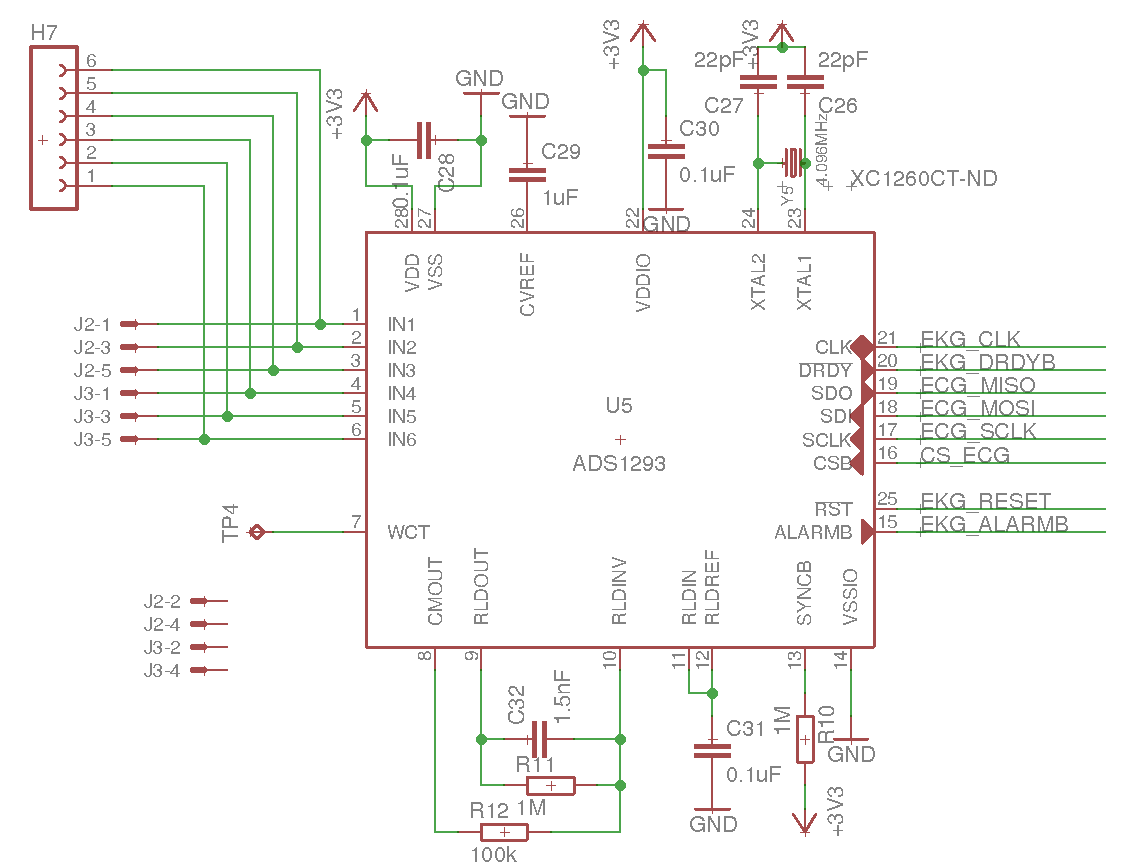
\includegraphics[scale=1,width=0.8\textwidth]{Images/Rev5_ECG.png} 
		\caption{ECG connections for Whip Sensor}
	\end{center}
\end{figure}

The previous WHIP prototypes made use of instrumentation amplifiers and op amps. Designs had begun to allow for adjustable gain via digitally controlled potentiometers in the feedback circuit. However, as designs were progressing a monolithic IC was released that provided all the features required in a single IC package, the ADS1293.\cite{ADS1293} This ECG front-end provides a full analog solution with software adjustable gain for up to 5 leads with Right Leg Drive (RLD). The data interface is SPI compatible and fully interrupt driven with programmable data rates. The module does require its own crystal to operate correctly. ECG lead connectors were the only other module component. ECG connectors were chosen to interface with traditional hospital leads, but were ultimately removed in favor of the snap on solution discussed in \Cref{sec:EnclosureDesign}. Hospital leads were used heavily during prototyping and validation only. Software setup of th ECG module is provided in detail in \nameref{chap:SensorConcepts}, but results in an initial configuration by the control module at power up and then provides an interrupt driven stream of data to the control module until signaled to halt.

\subsubsection{The \spo2 module}

\begin{figure}
	\begin{center}
		\label{fig:Rev5_SPO2}
		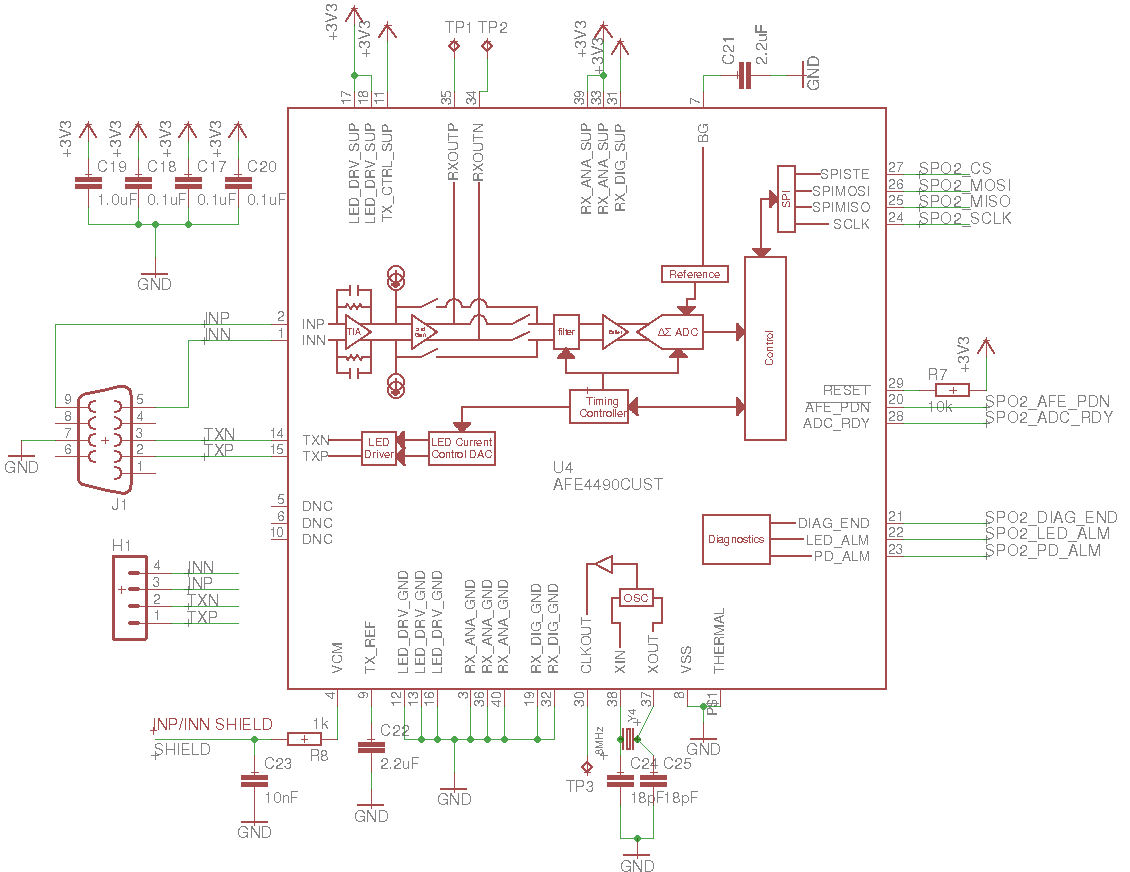
\includegraphics[scale=1,width=0.8\textwidth]{Images/Rev5_SPO2.png} 
		\caption{\spo2 connections for Whip Sensor}
	\end{center}
\end{figure}
Similar to the ECG module the discrete component implementation of the \spo2 module was replaced with a monolithic device, the AFE4490.\cite{AFE4490} The AFE4490 handles the signal multiplexing of both Red and IR LEDs, and allows software programmable gain, also over an SPI data bus. Also, like the ECG module IC the AFE4490 requires its own crystal. The last thing to mention about the \spo2 module shown in \cref{fig:Rev5_SPO2}, is the connector. The first analog PCB featured a through-hole DB9 connector was used to interface with the finger clip sensor, in subsequent designs a surface mount component was used instead. This introduced an unexpected point of failure when combined with the final PCBs and is addressed in \nameref{sec:EnclosureDesign}. The \spo2 module is provided an initial configuration by the control module at power-up and the provides and interrupt driven stream of data to the control module until told to halt.

\subsubsection{The Communication Module}
\begin{figure}
	\begin{center}
		\label{fig:Rev5_BT}
		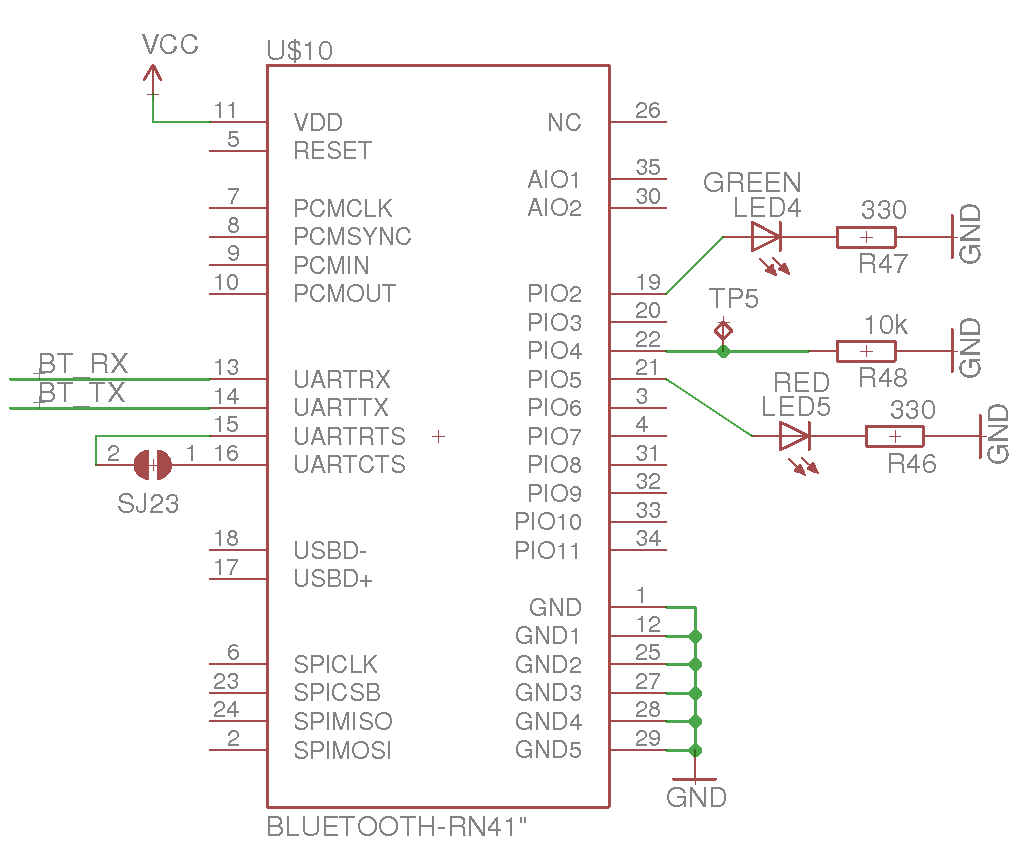
\includegraphics[scale=1,width=0.8\textwidth]{Images/Rev5_BT.png} 
		\caption{Bluetooth Serial Communication connections for Whip Sensor}
	\end{center}
\end{figure}
The communication module implements a black box full duplex asynchronous serial connection with another device over Blue tooth. this modules design was validated in revision one and has remained unchanged since that time. 

\subsubsection{The Control Module}
% "of the Whip" - "of the Wireless Health indicator Patch"
The control module is the main brain of the WHIP. The Atmel AT32UC3B0512C provides multiple SPI channels with hardware DMA access, a full floating point calculation unit, full speed USB hardware stack, and a serial link for the communication module.\cite{AT32UC3B} The processor is new in this revision, but the UC3 family has been used for all prototypes. Additionally, since the firmware for this device was written using the Atmel Software Framework (ASF) as a hardware abstraction layer, almost all firmware code written previously was easily ported to the new processor. Due to size, the schematic for the control module has been put in \nameref{fig:FullSchematic_Sheet1}.

\subsubsection {Sub-Module Design and Testing}

\begin{figure};
	\begin{center}
		\label{fig:Breakouts}
		\includegraphics[scale=1,width=0.45\textwidth]{Images/ECGBreakout.png} 
		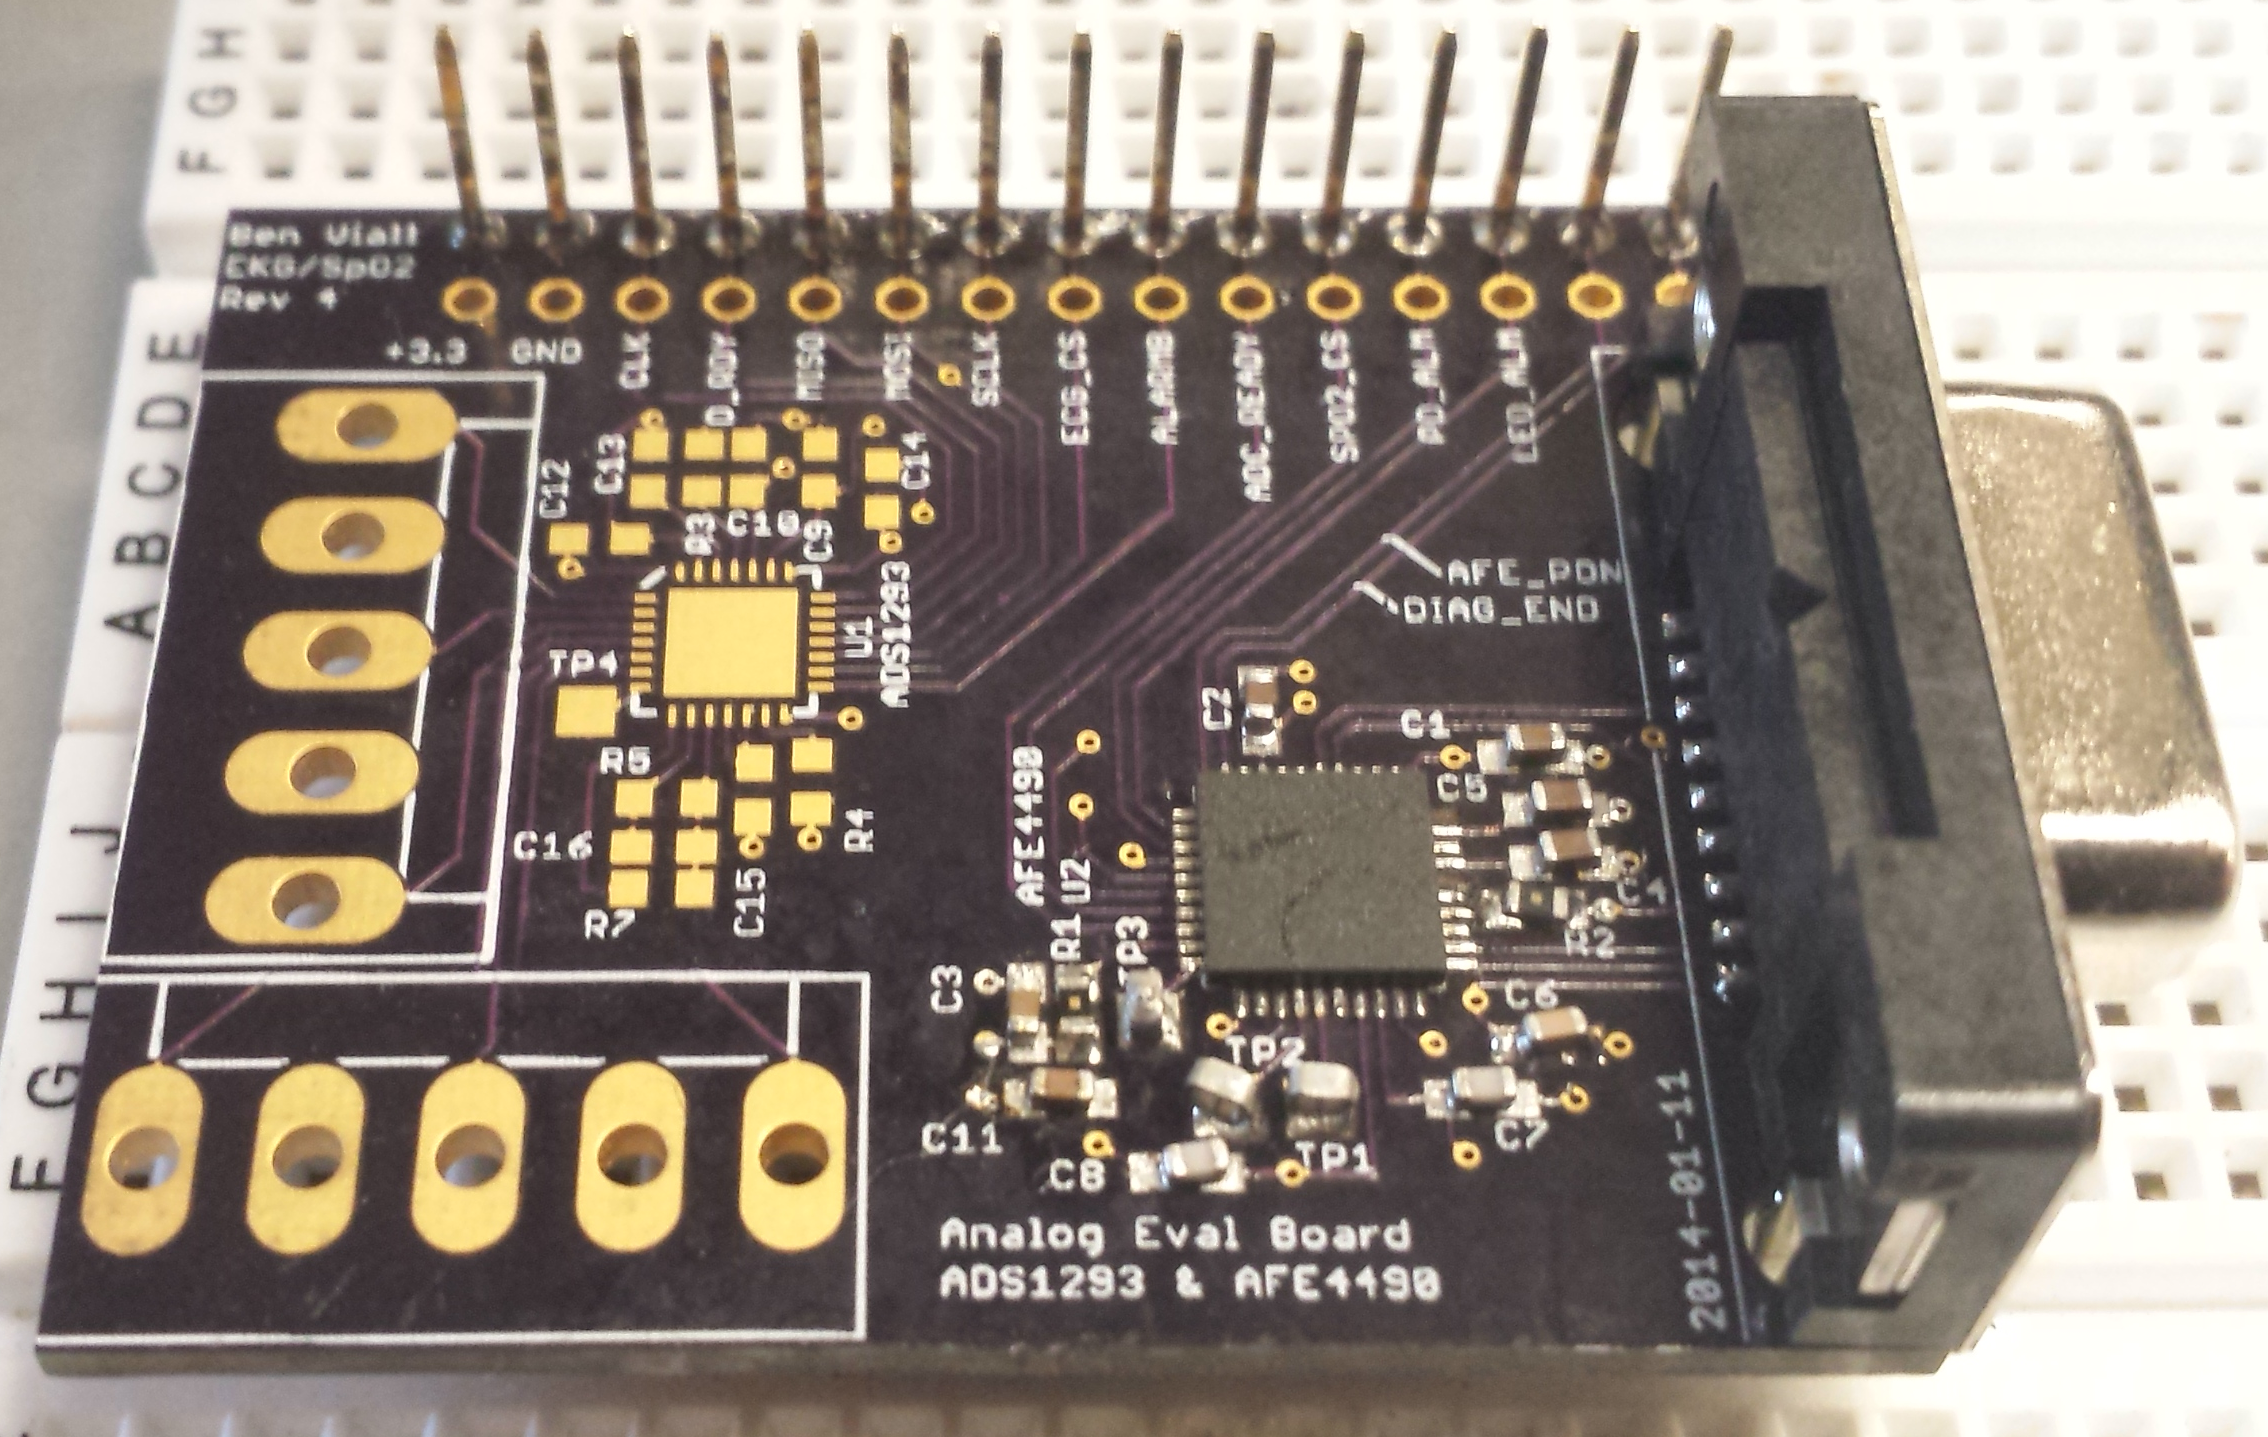
\includegraphics[scale=1,width=0.45\textwidth]{Images/SPO2Breakout.png} 		
		\caption{Populated Breakout Boards for ECG and \spo2 devices}
	\end{center}
\end{figure}

Time is always a factor in any production, to start the trial as soon as possible integration was done in only two steps, first the ECG and \spo2 Modules were fabricated to a PCB and confirmed to meet requirements. This type of PCB is often referred to as a breakout board. The signals are brought from a tight pin pitch device to 0.100 inch headers for breadboarding. An ATMega32U4 \cite{ATMEGA32U4} was tasked with supplying configuration data to the analog front end chips, then consuming the data as it was delivered for basic testing of the design. A basic heart monitor was created as proof of concept to showcase the validity of the design by adding an OLED module to display a real-time EKG shown in \cref{fig:Breakout Test}. This design was brought to the UMASSD fitness center, where it survived a burn in test on a subject running on a treadmill for approximately 30 minutes. 
The treadmill test utilized version two of the breakout board since the first breakout PCB demonstrated a serious problem with the artwork for the \spo2 module; the AFE4490 chip didn't fit in the space provided. Another revision was sent for production while work continued with the ECG. The advantage of creating a breakout board for the two modules was in the freedom to confirm every connection. Several of the control and status signals were unclearly documented. Once the breakout board arrived, the signals could be experimented with, using hookup wire. Despite the problems with PCB artwork on the breakout board, ultimately fabricating breakout boards saved both time and money, because the footprint error was discovered earlier in the design process.

\begin{figure};
	\begin{center}
		\label{fig:Breakout Test}
		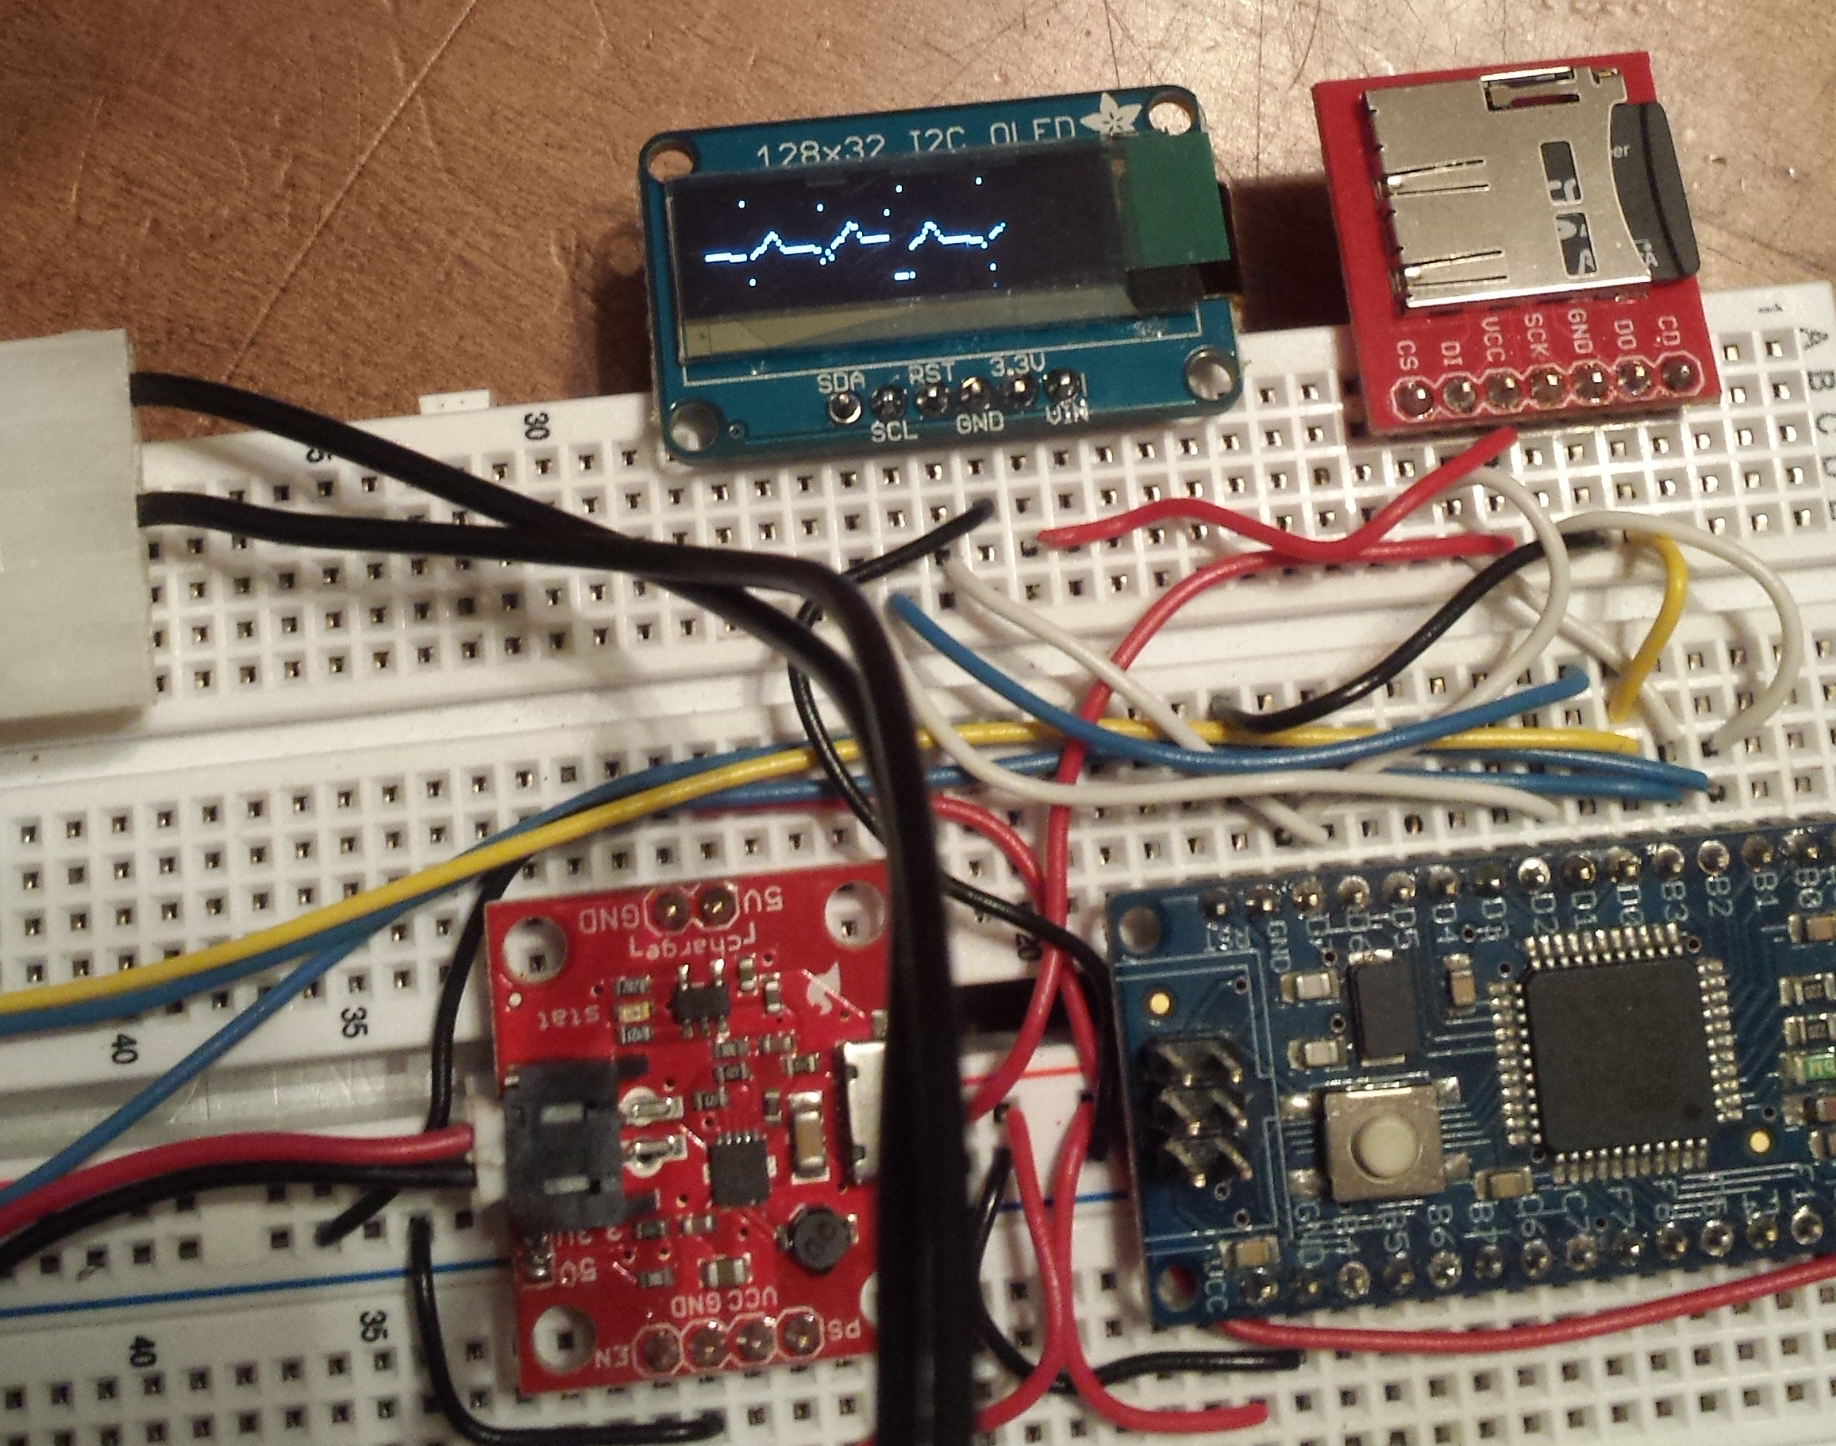
\includegraphics[scale=1,width=0.45\textwidth]{Images/BreadBoardTest.png} 		
		\caption{Test Rig For ECG and \spo2 Breakout Board showing real-time ECG trace}
	\end{center}
\end{figure}


\subsection{Printed Circuit Board (PCB) Layout}
After all modules had been designed in schematic capture, the design for the PCB began. The physical location of connectors was the driving force in the layout process. Given the board manufacturer in use at the time of production, the physical size of the board was set to 100 mm by 50 mm. The ECG and \spo2 transducer connections as well as the USB and SD card port were required to be on the board perimeter. Each module had its components grouped near each other and were routed to the module level. The modules were then positioned near their final destinations and inter-module routing occurred. the final Layout is shown in \Cref{fig:FullLayout}.

\begin{figure}[ht]
\begin{center}
	\label{fig:FullLayout}
	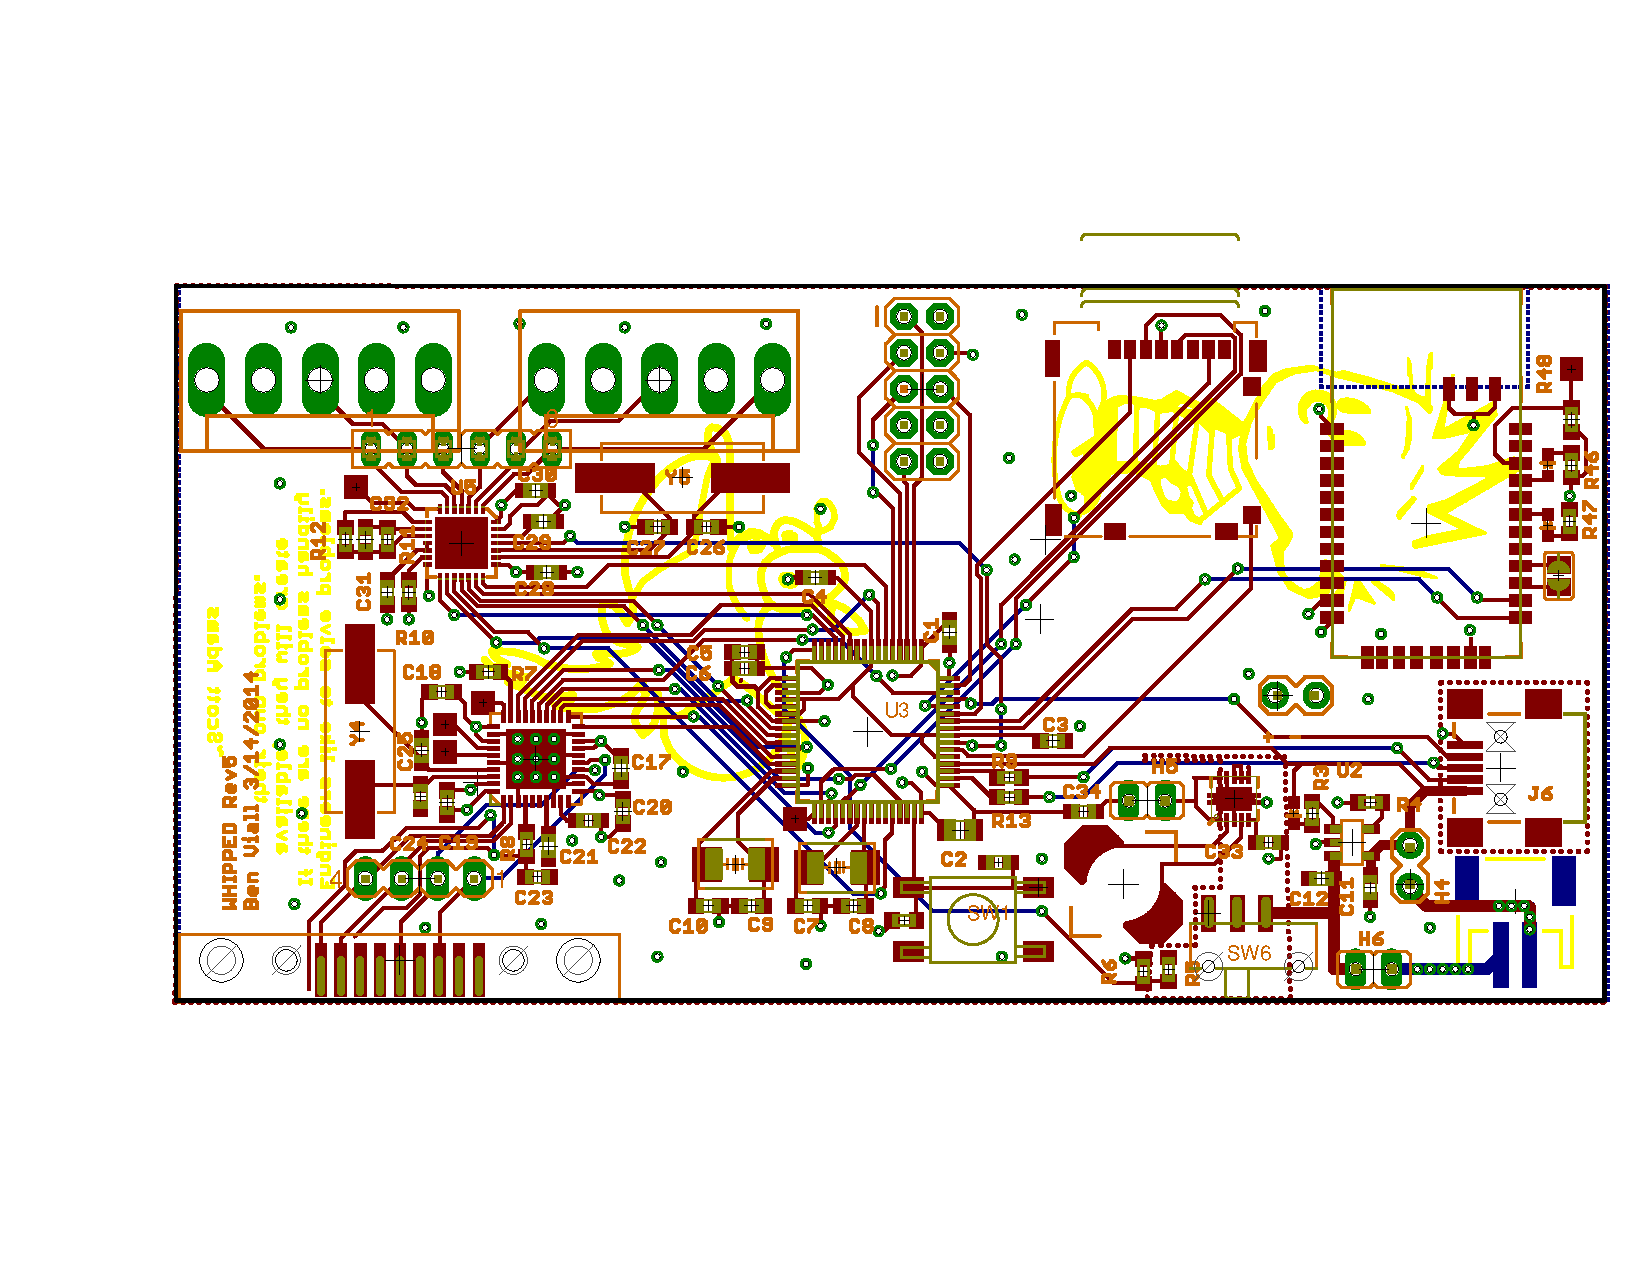
\includegraphics[angle=0,scale=1,width=1\textwidth]{Images/rev1D_PCB.pdf} 
	\caption{Full Layout Top and Bottom}
\end{center}
\end{figure}

Some modules in the WHIP design required special consideration beyond what could be recorded during schematic capture. The bluetooth module required the antenna to have no traces or copper pour beneath it's antenna area. this pullback can be seen on the upper right corner of all gerber layers in  \Cref{chap:PCB_LAYOUT}: \nameref{chap:PCB_LAYOUT}. Also, theSD module's physical placement was very sensitive; and needed to be placed close enough to the edge of the board to allow for card ejection but far enough away to prevent accidental ejection. Finally, the \spo2 module application note recommended gaurd traces to prevent noise that were routed around the sensitive signal traces. 


\subsection {Final Prototype Construction}
The second stage of integration occurred on the final WHIP PCB. Unlike production PCB assembly, the first prototype was not assembled all at once. First the power module was soldered together, and tested with a multimeter. This supply must have a load to provide proper regulation, therefore a 10,000-Ohm resistor was bridged across VCC and GND. The power system was validated as working only after adding this load resistor and confirming 3.3 Volts. The charging system was then validated by plugging a partially drained LIPO battery into the board with a USB cable connected to a computer. If the indicator 'LED1' lights, the charging circuit is validated. 

Now that the entire power module is soldered all other tests are prefaced by an additional test. Before reapplying power after any soldering, a multimeter should be used to check for accidental shorts between VCC and GND. Additionally, it is often useful to perform the "finger test" when powering new peripherals. The finger test involves placing a finger on the top of an IC package as you power the PCB. If there is an error in soldering, or wiring, the chip will, more than likely, heat up, your finger can detect this thermal event and power can be disconnected, hopefully before any damage is done, either to your power supply,your finger, or your new component. These tests will not be mentioned in the descriptions below, but are still performed before power is applied during every test.

The communication module was next to be validated, after removing all power, the communication module is added to the PCB. When power was applied, an attempt was made to connect to the module using an android phone. If pairing is successful, an additional test is performed. Opening a serial communication terminal on the phone "+++" is sent across the link if the module responds with "OK" then the Bluetooth module has entered over the air (OTA) configuration mode. Power can now be removed and the control module and Memory Module can be soldered on. 

The remaining tests all involve running parts of a validation firmware. The firmware runs on the microprocessor and exercises each of the other modules and provides an automated readout on the serial port. The JTAG module inside the microprocessor must be running o run the remaining test. This is tested by attaching the JTAG programmer to the board and attempting to read the device ID. if the test fails there is likely a soldering error, such as two or more pins shorted together, or a pin the is not soldered directly to the pad. A multimeter in continuity mode can find these errors quickly. 

\begin{figure}[ht]
\begin{center}
	\label{fig:ECG_Test_Pass}
	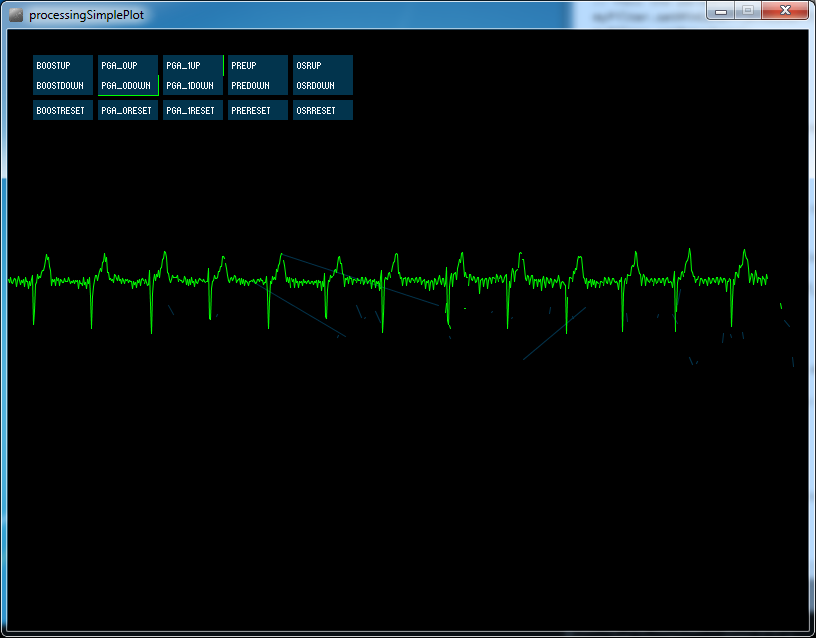
\includegraphics[angle=0,scale=1,width=1\textwidth]{Images/ECG_processingSketch.png} 
	\caption{Successful test of 'ECGcheck' firmware}
\end{center}
\end{figure}

Once firmware can be loaded into the microprocessor, insert an SD card into the device, power does not need to be removed. Run the SDcardcheck firmware and observe the serial output. The test will have PASS/FAIL result. Upon getting a PASS, disconnect the power and solder the \spo2 Module, and load the SPO2check firmware and the PC side software. Connect the finger clip to the board and affix it to your finger. Connect the PC software to the device via the local COM port and hit run. You should see a two graphs representing your Red and IR Photoplethysmograph. Finally, disconnect the power.

Finally, solder the ECG module to the PCB. Load the ECGcheck firmware and accompanying PC side software. Connect the 3 ECG leads to a patient or other signal source. Connect the PC software to the device via the local COM port and hit run. You should see a rolling graph of your ECG similar to \cref{fig:ECG_Test_Pass}. Now, all components should be on the board, and have been validated.


Once the first prototype was validated, six boards at a time were populated at once. First solder paste was applied to all boards using a stencil. Then, all components were manually populating. Finally, the boards were soldered in a custom made reflow oven. The results are shown in \cref{fig:ReflowedBoards}. Each board was then checked for shorts and reworked as needed.

\begin{figure}[ht]
\begin{center}
	\label{fig:ReflowedBoards}
	\includegraphics[angle=0,scale=1,width=1\textwidth]{Images/BoardsSoldered.png} 
	\caption{Fully populated boards, just out of the reflow oven}
\end{center}
\end{figure}


\section {Enclosure Design}
\label{sec:EnclosureDesign}
Part of the research component of this dissertation was to evaluate methods, and make design choices, to promote the usability of the  proposed technology; specifically to encourage adoption by people over the age of 65. The next step in the integration process was to create an apparatus, that could be easily put on by a patient and provide reliable positioning of the electrodes every time. An important requirement of the physical design was to provide long term wearibility, the device should be worn anytime the user is awake. One exception is any time the device may be exposed to water. Deciding the device not be waterproof for the current trial simplified the design. The first goal of the enclosure, then, was to make it as comfortable as possible while maintaining overall functionality. The apparatus was designed in two parts: the chest strap, and the electronics enclosure. 




\subsection {Chest Strap}
\begin{figure}[ht]
\begin{center}
	\label{fig:Electrodes}
	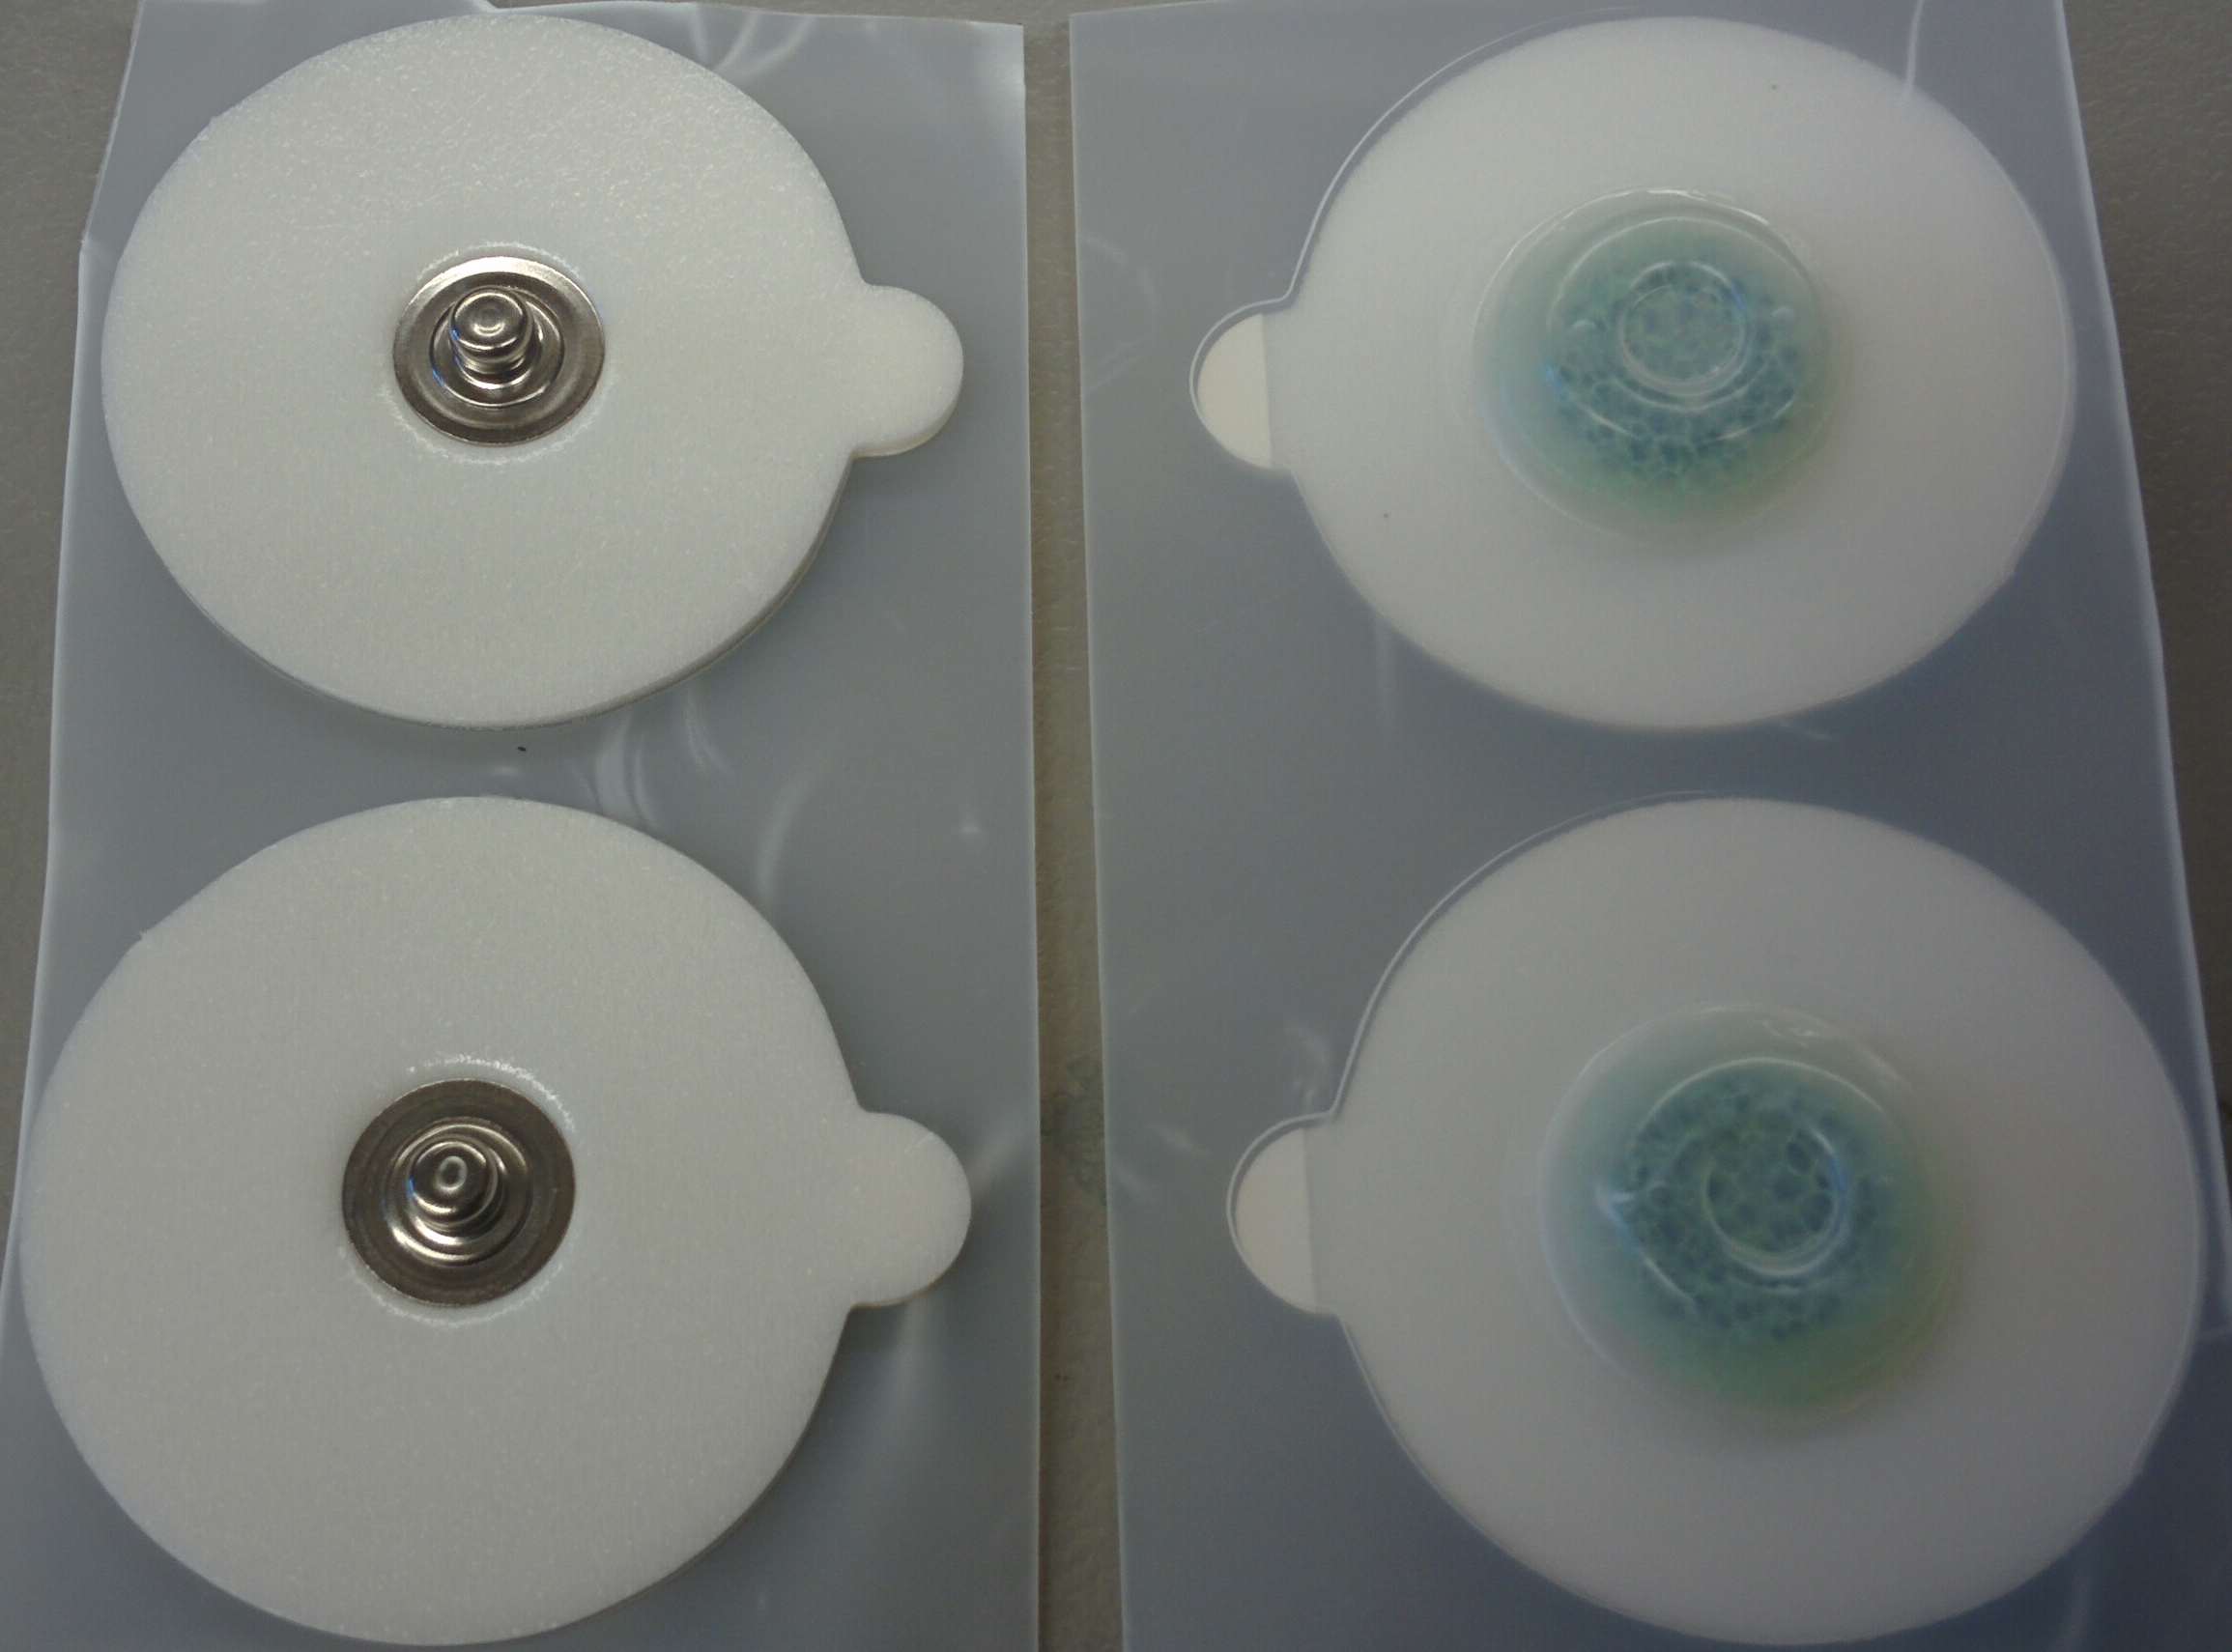
\includegraphics[angle=0,scale=1,width=.5\textwidth]{Images/Electrodes.png} 
	\caption{Sticky Electrodes, top and bottom}
\end{center}
\end{figure}
Initial testing of the device was performed in a laboratory setting using a sensor board equipped with rubber feet to prevent shorting any exposed traces on the underside of the PCB. A temporary cable was constructed the connected to traditional pre-moistened sticky electrodes shown in \cref{fig:Electrodes}. This design was scrapped after areas of irritation began to appear on the engineers after several days of ripping off and reapplying electrodes. It was clear that wet electrodes would not be appropriate for long term use.

The next design replaced sticky electrodes with dry contacts held in place by means of a stretchable fabric strap. Each strap was fitted with a buckle to make it easy to both put on and take off. Three electrodes, made of velostat, a conductive flexible material often found in commercial fitness bands, were sewn into the strap and connected with fabric snaps to the sensor board. This design functioned well electrically, however no fabric could be sourced that offered the correct combination of traits to make it both feel comfortable, and support the sensor board. This metric, of feeling comfortable, was qualitative only. No quantitative data on feel was collected during the design process.

After several iterations, that never produced a qualitative approval by testers, off the shelf straps designed for runners, specifically the polar heart rate monitor strap was used. The heart rate sensor hardware made by polar was not used, only the strap. The polar strap provided a comfortable feeling strap that could also support the weight of the sensor board and battery. However, these straps only provided two electrodes. A third electrode was added using the velostat material from the second prototype. The final strap connection is shown in \cref{fig:polar_3rdSnap}.

\begin{figure}[ht]
\begin{center}
	\label{fig:polar_3rdSnap}
	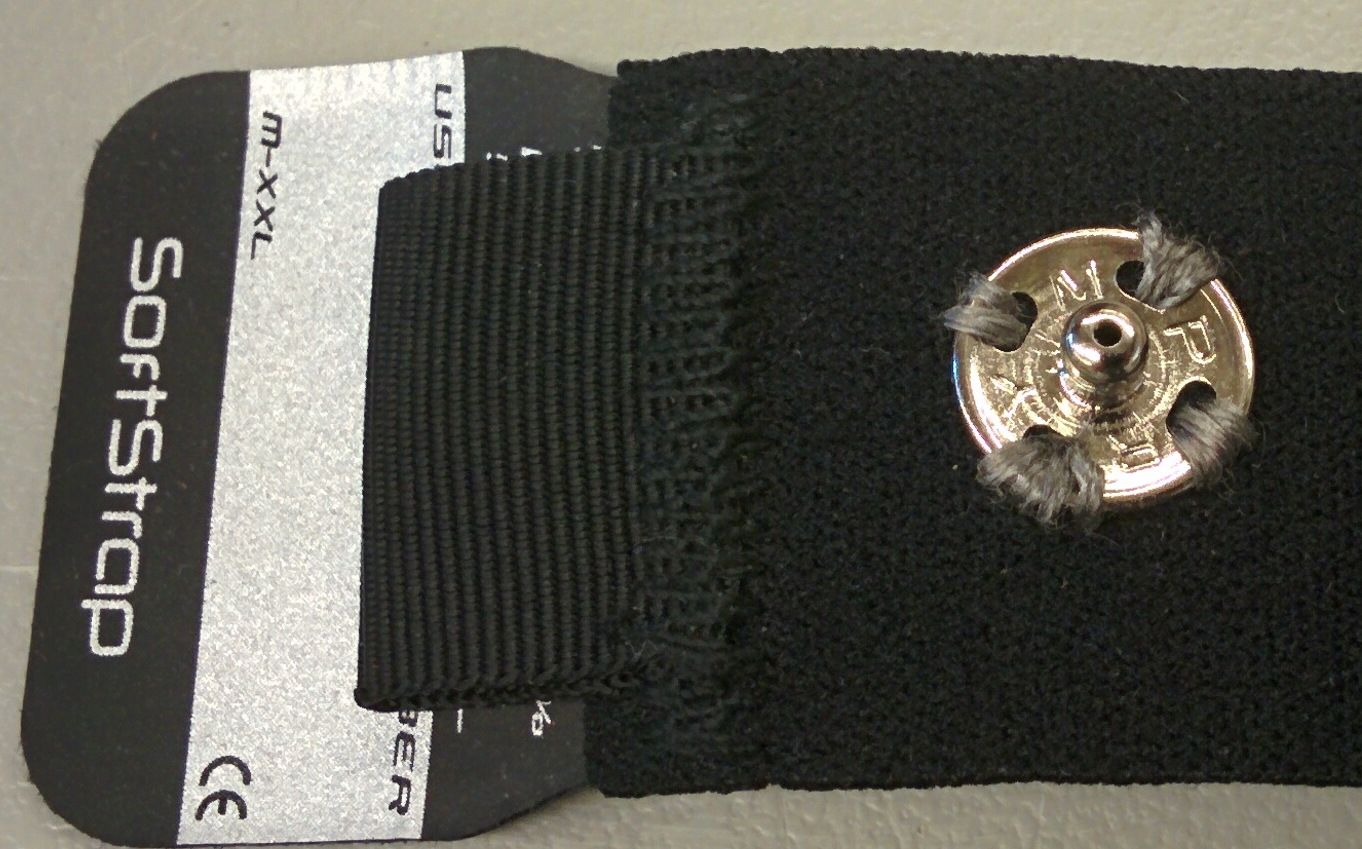
\includegraphics[angle=0,scale=1,width=.51\textwidth]{Images/Polar_top.png} 
	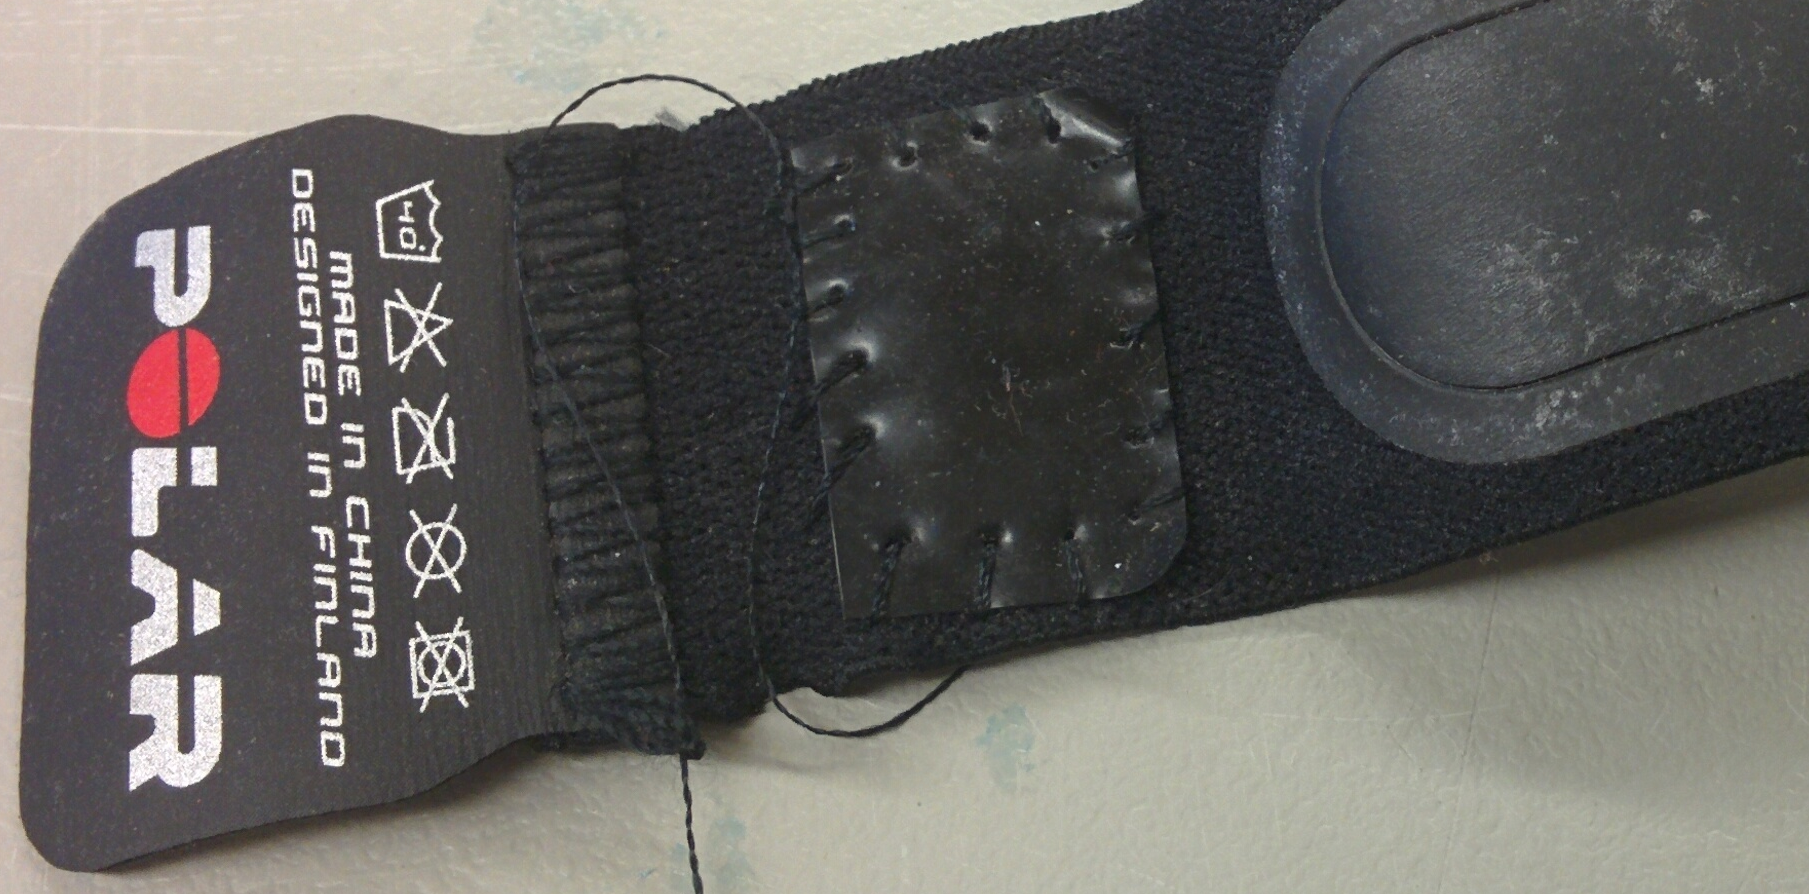
\includegraphics[angle=0,scale=1,width=.51\textwidth]{Images/Polar_bottom.png}
	\caption{Third Electrode, Sewn using conductive thread and fabric}
\end{center}
\end{figure}

 

\begin{figure}[ht]
 \begin{center}
  \label{fig:PCBvsRender}
  \includegraphics[scale=1,width=0.8\textwidth]{Images/Rev5Assembled.png} 
  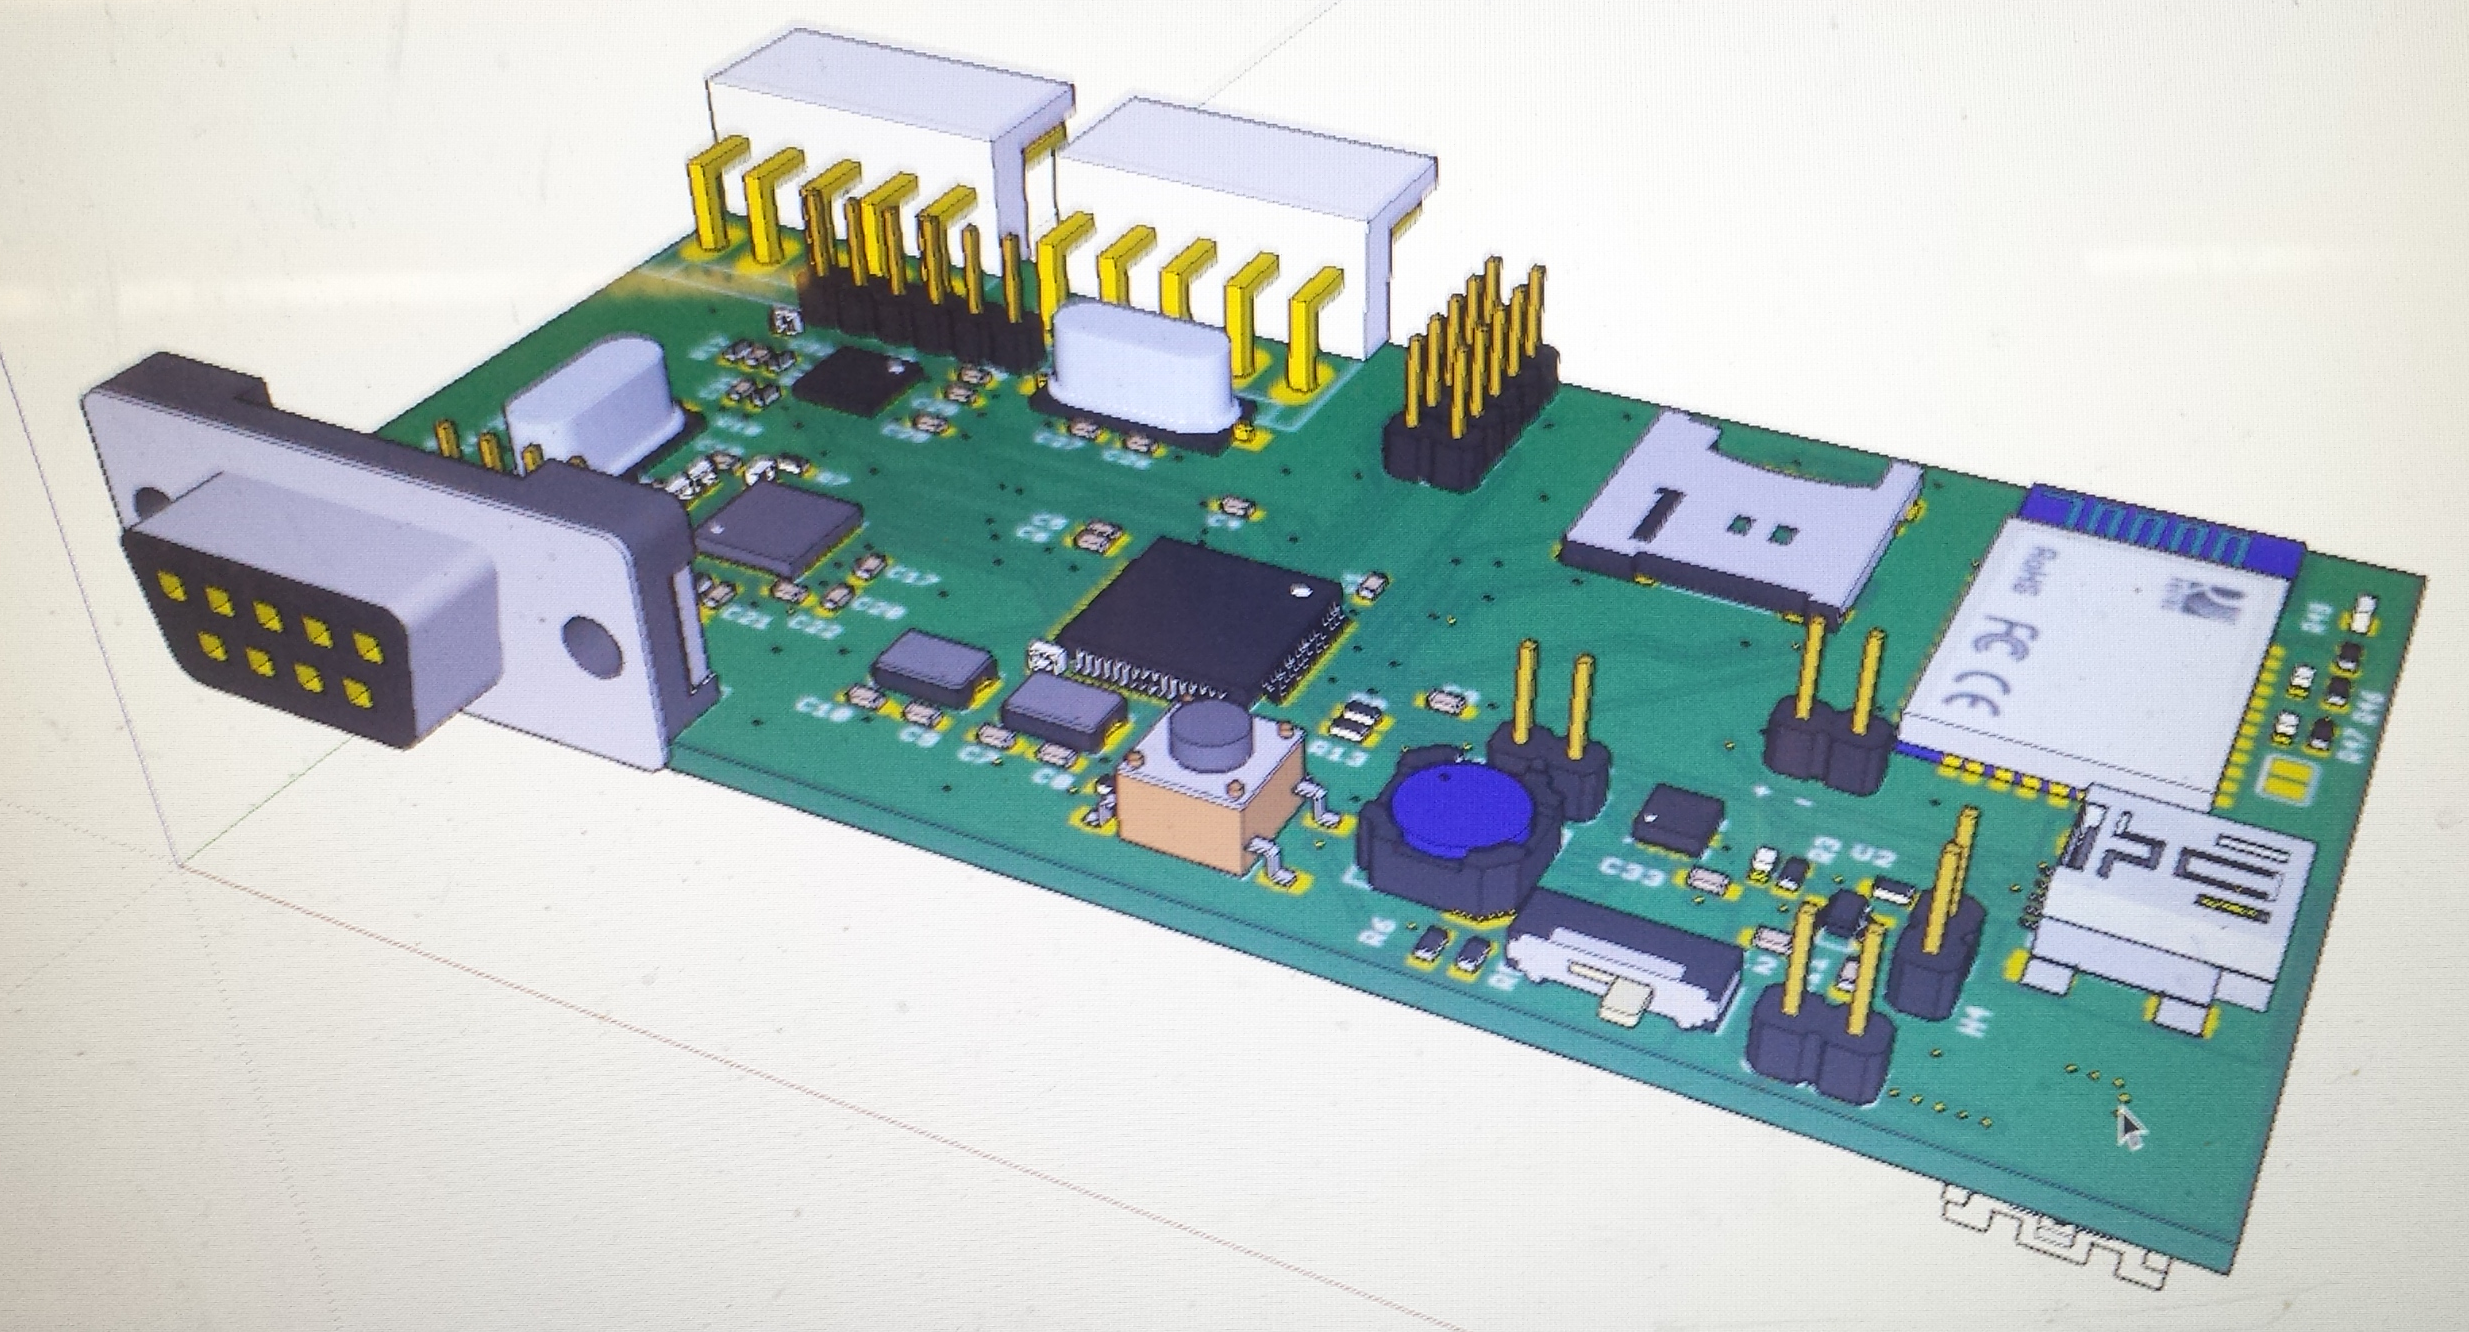
\includegraphics[scale=1,width=0.8\textwidth]{Images/Rev5_prerender.png} 
  \caption{Populated PCB versus 3d Render}
 
 \end{center}
\end{figure}

\subsection {3d printed enclosure}
The electronics enclosure served several purposes, first protecting all sensitive components from external damage. Second, providing clear access to ports of interest, including: charging port, sd card, ECG, and \spo2 ports. Lastly, keeping all components of the design enclosed together physically. 

All enclosure designs were 3d printed. 3d printing takes a digital 3d model and creates a physical object, either out of an extruded material such as plastic or wood, a process known as Fused Deposition Modeling (FDM), or by repeatedly adding a thin layer of small particles,or resin, and using a laser to selectively melt those particles to the component underneath (SLS). Both methods are common in prototyping and each has its own advantages that are not the focus of this dissertation. A Lulzbot Taz4 \cite{LULZBOT} was used to create the models used in this dissertation. The Taz4 is a FDM type machine, all models were created out of Acrylonitrile butadiene styrene (ABS) plastic. ABS was chosen for its high strength properties. 3d printing the enclosures allowed us to rapidly change the design, sometimes several times a day, and get immediate physical feedback on the design. There is no clear number of how many prototype stages were used in the design as a result. However, the following paragraphs will explain the design decisions made,from first prototype, to final prototype enclosure.


First we should discuss how the enclosure was designed. All models were created using SketchUp\cite{Sketchup}. The choice of modeling software stemmed from the existing PCB work-flow. EagleCad, the PCB design software used to make the sensor PCB, allows custom scripts or User Language Programs (ULPs) to automate tasks or augment features of the program, one available ULP allows an export of the board directly into SketchUp. The basic export only provides a 3d model of the PCB without any components on it. however, if a 3d model of each component type is available, a fully populated PCB is imported into SketchUp. A fully populated PCB model was used, not just for enclosure design, but also for checking the clearances between components before the board was fabricated. Substantial effort was put into creating 3d models of components based on the mechanical drawings from the component data-sheets. As shown in \Cref{fig:PCBvsRender} the fully populated board is well represented by the 3d model. Using a generated 3d model allowed the designer to provide tight tolerances for the overall enclosure design. 

The first enclosure was a simple box designed to hold the unpopulated PCB. Notable features of this first board included retaining clips above the board, rounded corners, integrated standoffs, and a compartment for the battery below the PCB. This was the first 3d printed object made for this project, and was used as a basic shakedown of the 3d printing process shown in . The utility of 3d printing was made immediately clear once the first prototype was printed. The PCB fit snuggly and did not move once seated. Indeed, once it was in it was difficult to get out. The second design change needed was to accommodate the battery. The standoffs were spaced too closely together to fit the battery. Testing this prototype required two standoffs be cut from the plastic model and can be seen on the left side of the enclosure in  \Cref{fig:enclosure1}. This "modify-after-print" approach was invaluable at each stage of the design.

\begin{figure}[ht]
 \begin{center}
  \label{fig:enclosure1}
  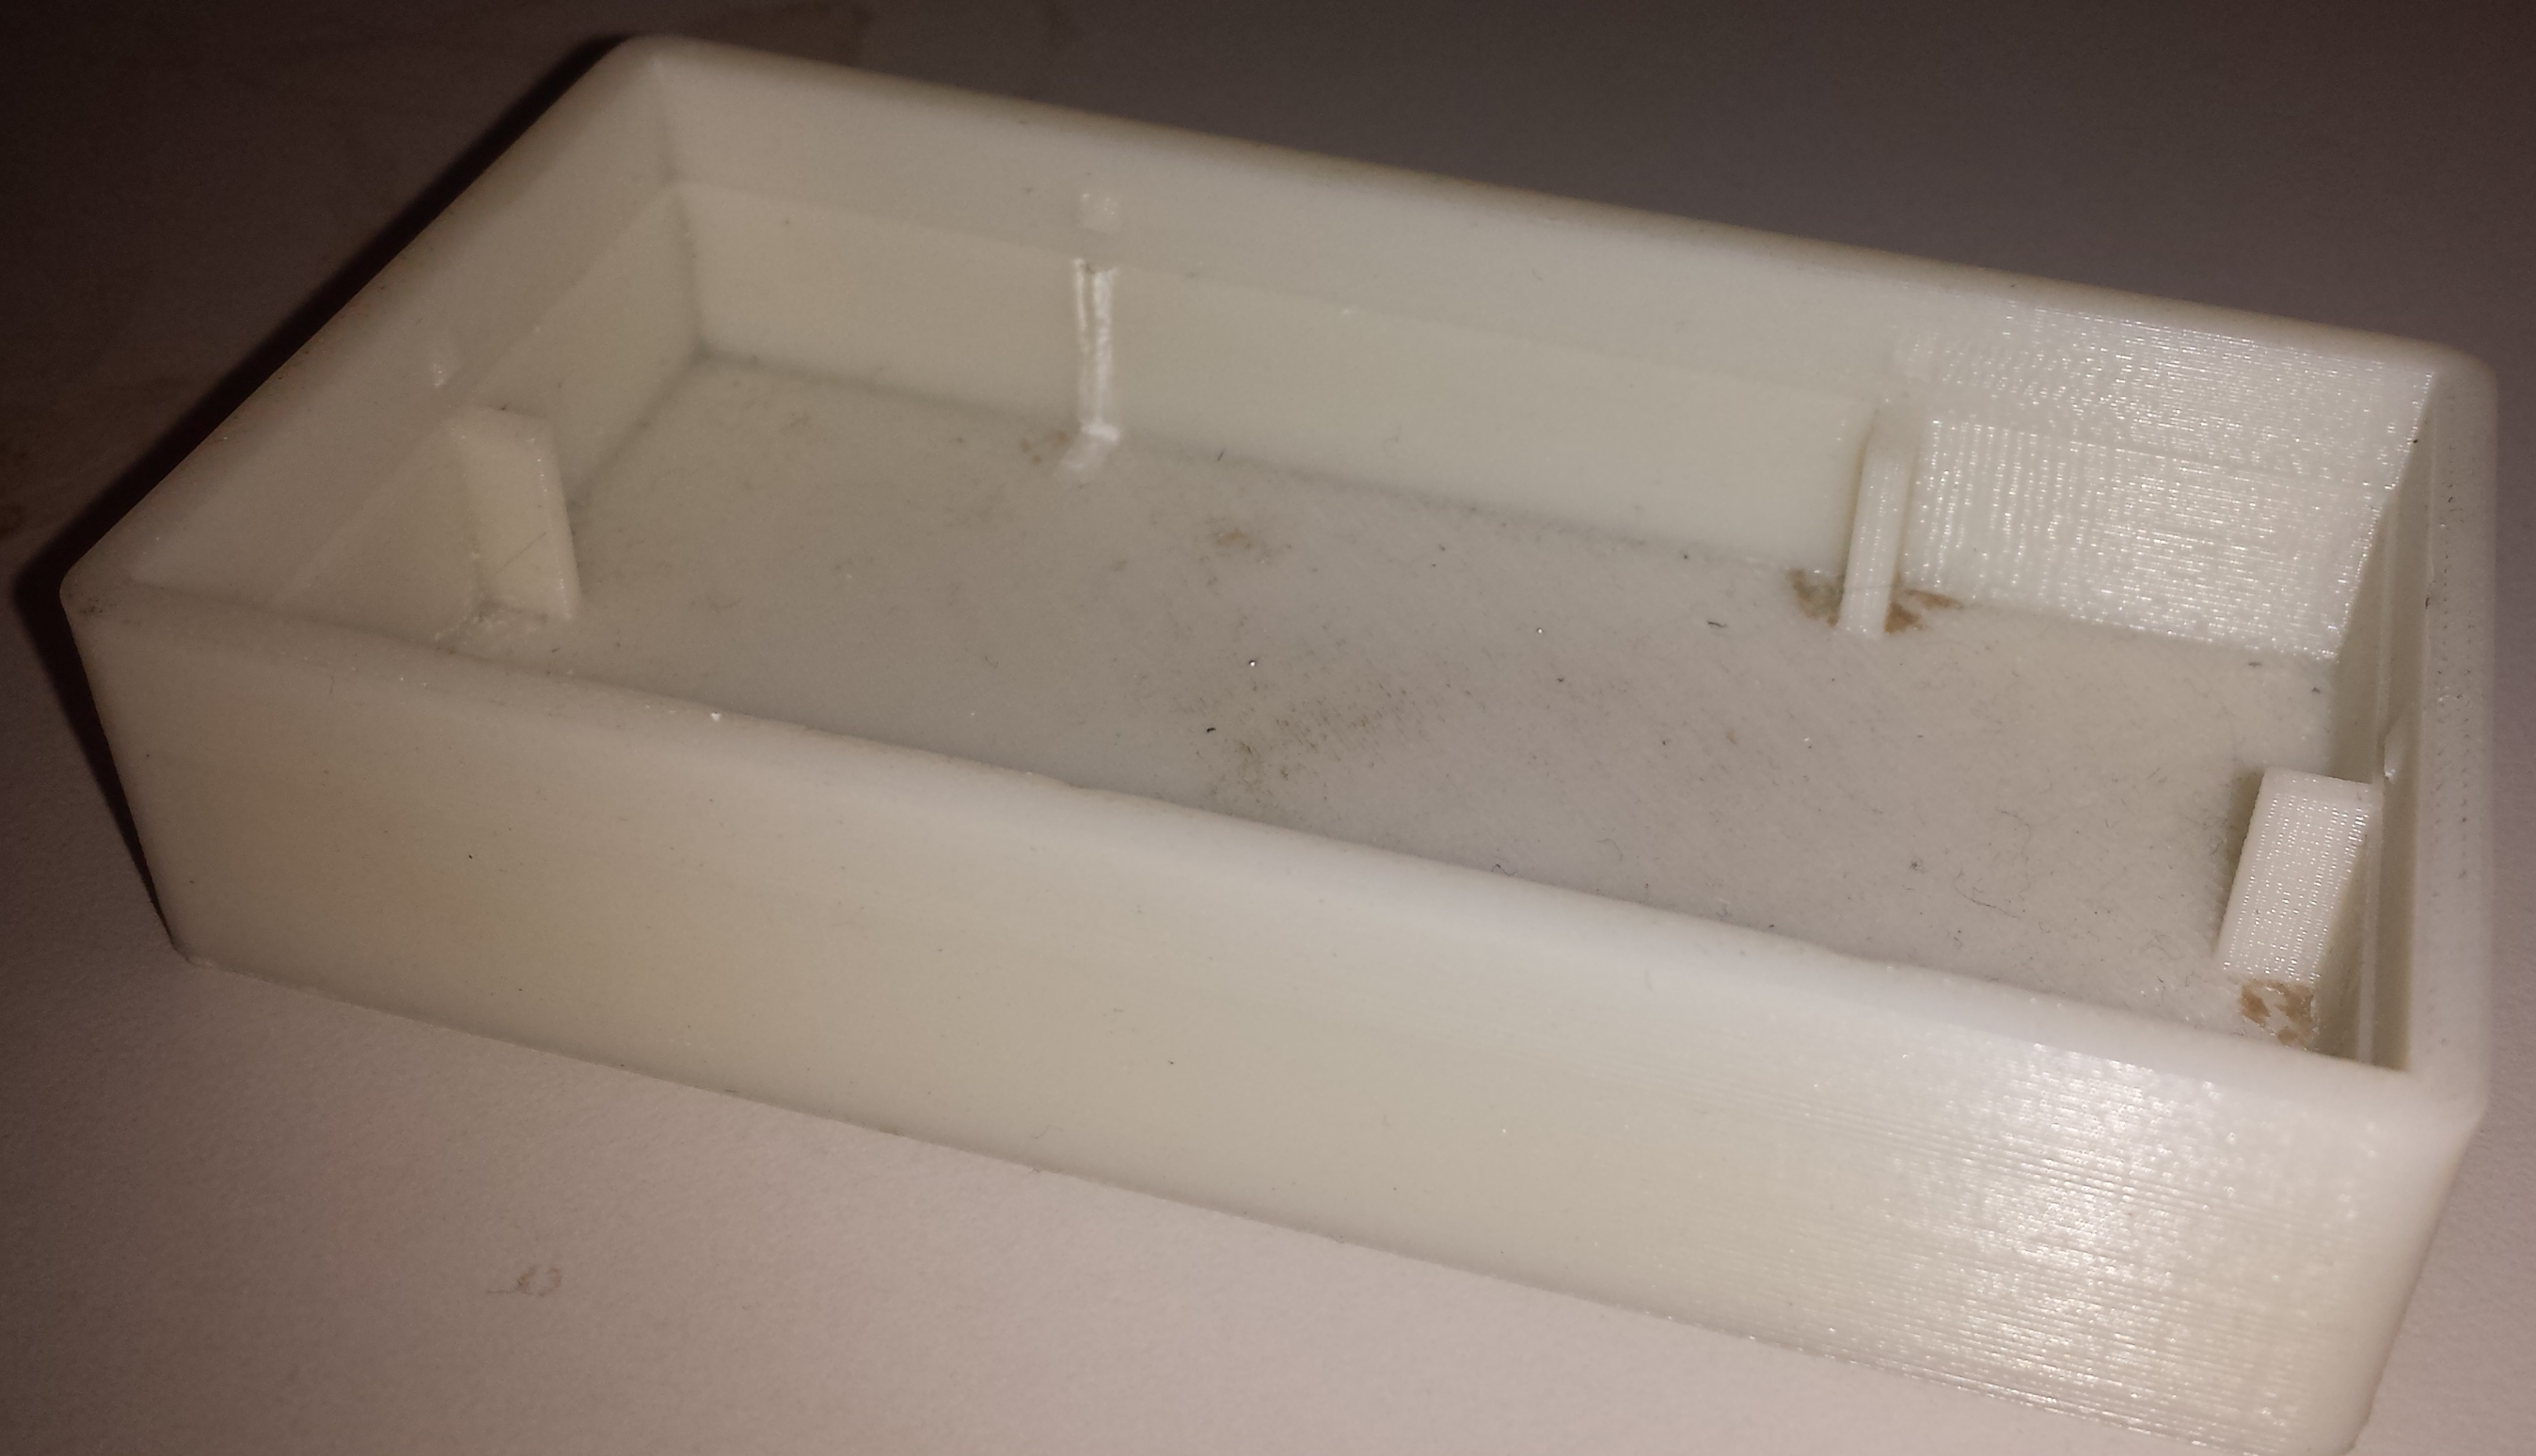
\includegraphics[scale=1,width=0.8\textwidth]{Images/Enclosure1.png} 
  \caption{Enclosure Rev1, with cut tabs}
 
 \end{center}
\end{figure}


The next prototype stage moved the PCB standoffs, added ports for the USB, SD card, \spo2, and ECG connectors. It also smoothed out not only the four vertical edges of the enclosure but rounded all four bottom edges as well. A cover was also printed to completely enclose the electronics. A portion of the cover was designed to prevent warping, but reduce overall plastic use, as a structural precaution. This prototype worked well, allowing relatively easy removal of the PCB while still holding the board tight, however the SD card slot was not large enough to allow a thumb or finger to trigger the ejection mechanism for the card. The cover functioned well, but only after a section of the cover was removed to provide space for the programming header.  A hot knife was used, in each case, to remove plastic until the desired form was achieved, then calipers were used to measure the effected areas and the 3d model updated to reflect the new measurements.
\begin{figure}[ht]
 \begin{center}
  \label{fig:enclosure2}
  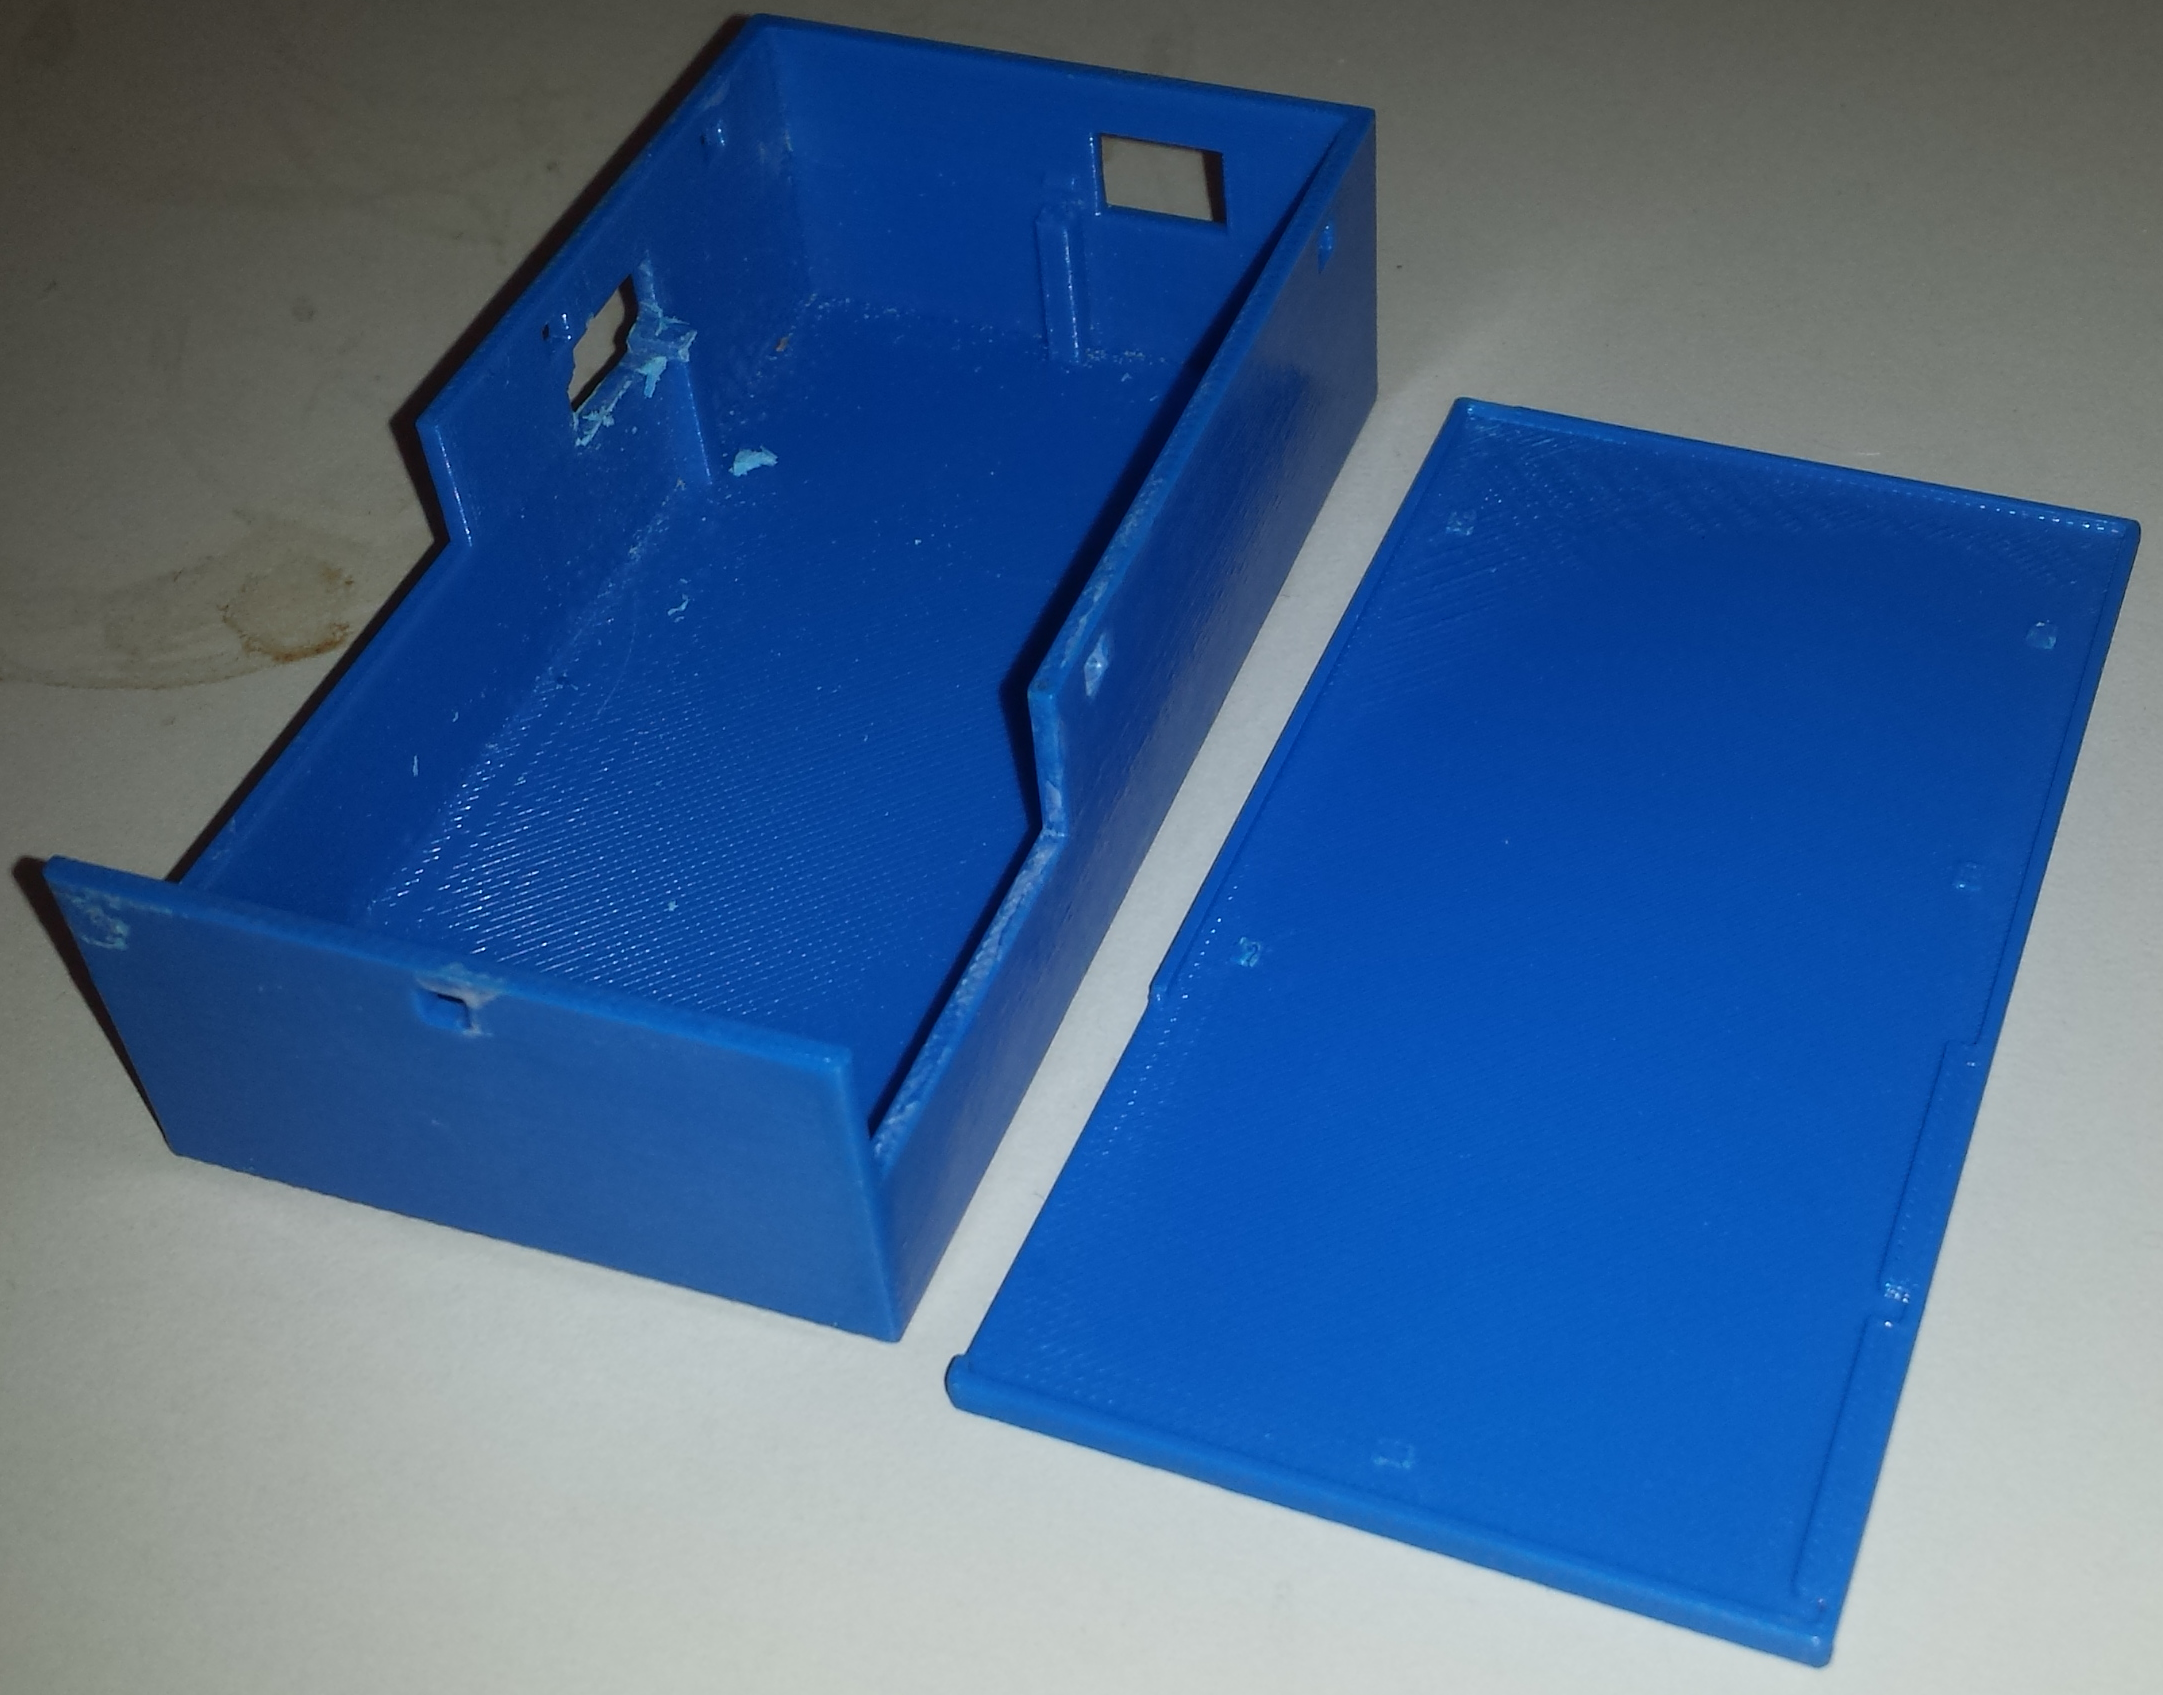
\includegraphics[scale=1,width=0.8\textwidth]{Images/Enclosure2.png} 
  \caption{Enclosure Rev2, with enlarged SD slot}
 
 \end{center}
\end{figure}


It was at this point in the design process that the polar heart rate strap was introduced. The next prototype moved the ECG connection port from the side of the device to the bottom. A small insert was fabricated to fit into the model to allow it to snap directly to the polar strap. This model was printed and again modified to make channels for the wires that would connect from the snaps to the PCB. As shown in \Cref{fig:enclosure3} the enclosure was actually modified twice, the first time the modifications were made while the enclosure was upside down, which brings to mind the old adage "measure twice, cut once". 

\begin{figure}[ht]
 \begin{center}
  \label{fig:enclosure3}
  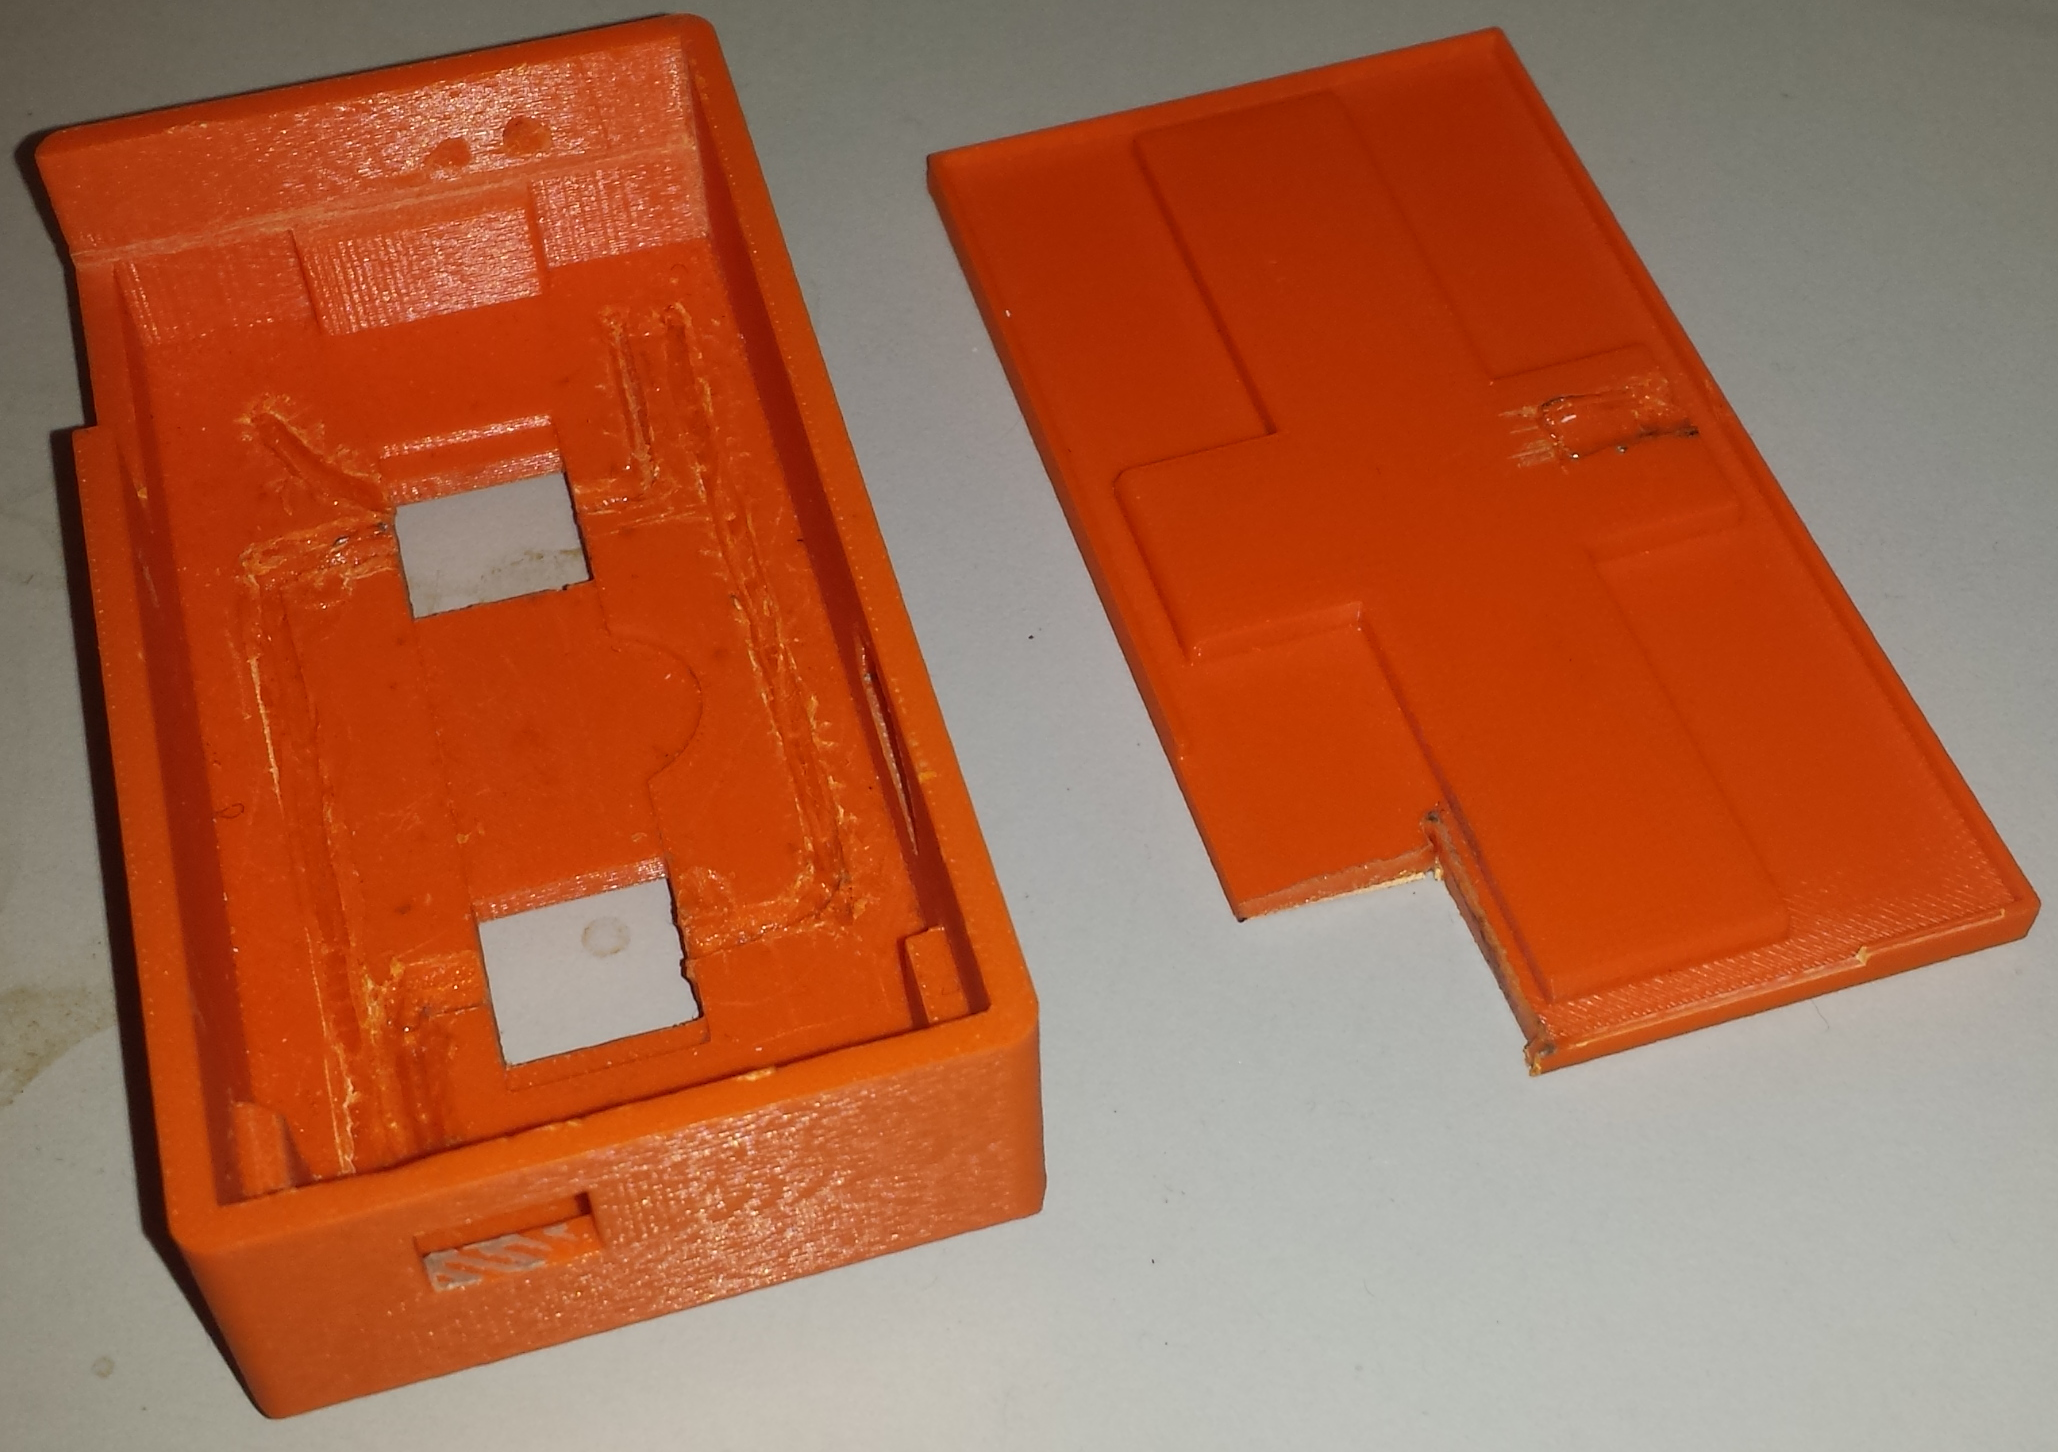
\includegraphics[scale=1,width=0.8\textwidth]{Images/Enclosure3.png} 
  \caption{Enclosure Rev3, with wire Management Trenches} 
 \end{center}
\end{figure}


The last enclosure integrates all the lessons learned in the previous designs, adding an extra aperture for the 3rd lead of the ECG. this design was printed multiple times for distribution during the study. The last modification to the enclosure was to put the entire device inside of a fabric pouch. The fabric was deemed more comfortable than the 3d printed plastic. Each fabric pouch was hand sewn and holes for the charging port and ECG leads were cut by hand. A hole for the SD card was not cut in the fabric to prevent accidental ejection during use. The fully constructed Enclosure is shown in \Cref{fig:enclosure4}.

\begin{figure}[ht]
 \begin{center}
  \label{fig:enclosure4}
  \includegraphics[scale=1,width=0.8\textwidth]{Images/Enclosure4.png} 
  \caption{Production Enclosure, with PCB and Battery} 
 \end{center}
\end{figure}

\subsection{enclosure conclusions}
3d printing was used to great effect in the enclosure design. The ability to modify a physical prototype provided the flexibility to just try design concepts on a whim. Since cost and risk are usually proportional in a design environment the extreme low cost of 3d printing, approximately two dollars and two hours per enclosure, provided a large amount of freedom to try out many designs before settling on a final implementation. Additionally, the ability to modify each prototype to add features allowed for instant feedback on each 3d model. 

The largest drawback to 3d printing each case was the time involved, and the rate of failure. The 3d printer was a new tool at the start of this process. Unfortunately it is not as user friendly as a traditional 2d laser printer. Going from model to printed object is not as simple as hitting "print". An additional step, know as Computer Aided Manufacturing (CAM), is required to turn the 3d model into movement instructions for the printer. This process is extremely flexible, however the flexibility provided by the process also introduces complexity. Additionally, to ensure reliable prints some preparation to the print bed is required. This was not immediately apparent, however once the problem was identified the rate of failure went from four out of five (80 \%) to one in fifty(2\%). A 2\% failure rate may be considered high in bulk manufacturing, but for prototyping, it is acceptable.


\begin{figure}[ht]
 \begin{center}
  \label{fig:enclosure5}
  \includegraphics[scale=1,width=0.8\textwidth]{Images/Enclosure5.png} 
  \caption{Enclosure with lessons learned} 
 \end{center}
\end{figure}

\subsection{Enclosure Future Work}
In future research, it may be possible to speed prototyping time by using subtractive manufacturing techniques. Using acrylic sheets and a laser cutter a similar enclosure design could be fabricated in minutes instead of hours. Future designs may also introduce flexible PCB material that would allow a smaller volume of the overall enclosure. Finally, a curved enclosure design would more closely fit to the patients body increasing comfort. A final Enclosure was fabricated addressing some problems discovered during the experimental trial and some limitations of 3d printing. The enclosure shown in \cref{fig:enclosure5} can be 3d printed without overhangs or support material and does not present a lip on the enclosure cover. Additionally, the cover has been modified to protect the \spo2 connector from torsional forces during use.







